\chapter{Time-resolved Core-scale Analysis of Fluid Displacement in an mixed-wet Carbonate}
 
The experimental fluid displacement process of brine and oil in a mixed-wetting Indiana limestone had been imaged by time-resolved synchrotron X-ray microtomography. The experimental protocols are described in Chapter three section 3.3.1, and summarised in table Fig.\ref{exps} first column. The displacement processes include 1)brine invasion of oil-saturated core, 2) oil re-injection into brine saturated core, 3) Steady-state injection of both fluids into oil saturated core. This chapter will show both qualitative and quantitative analysis on the experimental results based on tomography images.

\section{Pore space characterisation}
\subsection{Porosity: micro pores and macro pores}
In chapter 3, Fig.\ref{sempore} shows the SEM image of the topology of Indiana limestone pore space, and illustrates the macro and micro pores which size spans across few magnitudes. The macro/micro pores can be also identified on raw CT images. Fig.\ref{micropores} shows an example of micro pores that present as darker patches of shades in the rock. Although the micro pores are below CT spatial resolution, the micro-porous structure has a lighter bulk density that has less attenuation to the X-ray beam. As a result, the micro pores are identical on CT images although the exact topology is hard to define. Therefore estimation of porosity of micro pores can be roughly made. Nonetheless, it is still very difficult to investigate fluid occupation inside the micro-porosity. Due to this limitation, only the fluids that can be clearly identified in the macro pores were analysed in this thesis.

\begin{figure}[htbp]
  \centering
  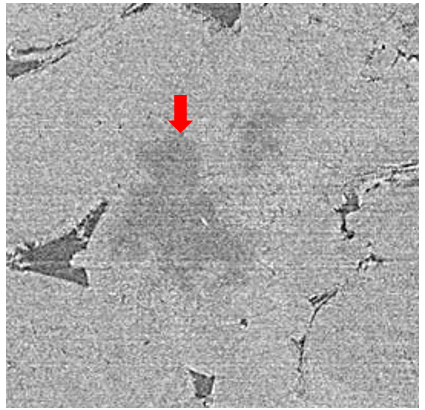
\includegraphics[width=0.7\textwidth]{\dir/figs/micropores.png}
  \caption{Indiana limestone}
  \label{micropores}
\end{figure}

\subsection{Pore size distribution}


\subsection{Representative elementary volume}
Representative Elementary Volume (REV) is the smallest unit volume over which measurements can represent the whole sample. Sample REV has to be at least no larger than the targeted volume to show representative result. REV is measured by step-wisely increasing the sampling size while measuring a bulk property for example porosity, the measurement will oscillate between the representative bulk value and then converge at average porosity that can represent the bulk when sample size is close to the REV. The REV of Indiana limestone was estimated using image-based porosity measurements across a range of volume sizes (Fig.\ref{rev}). The graph shows the porosity curve converges at 700 pixel (blue arrow), so the REV of this sample is ~3.65 mm$^3$ and well within the targeted volume which is ~15.55 mm$^3$.

\begin{figure}[htbp]
  \centering
  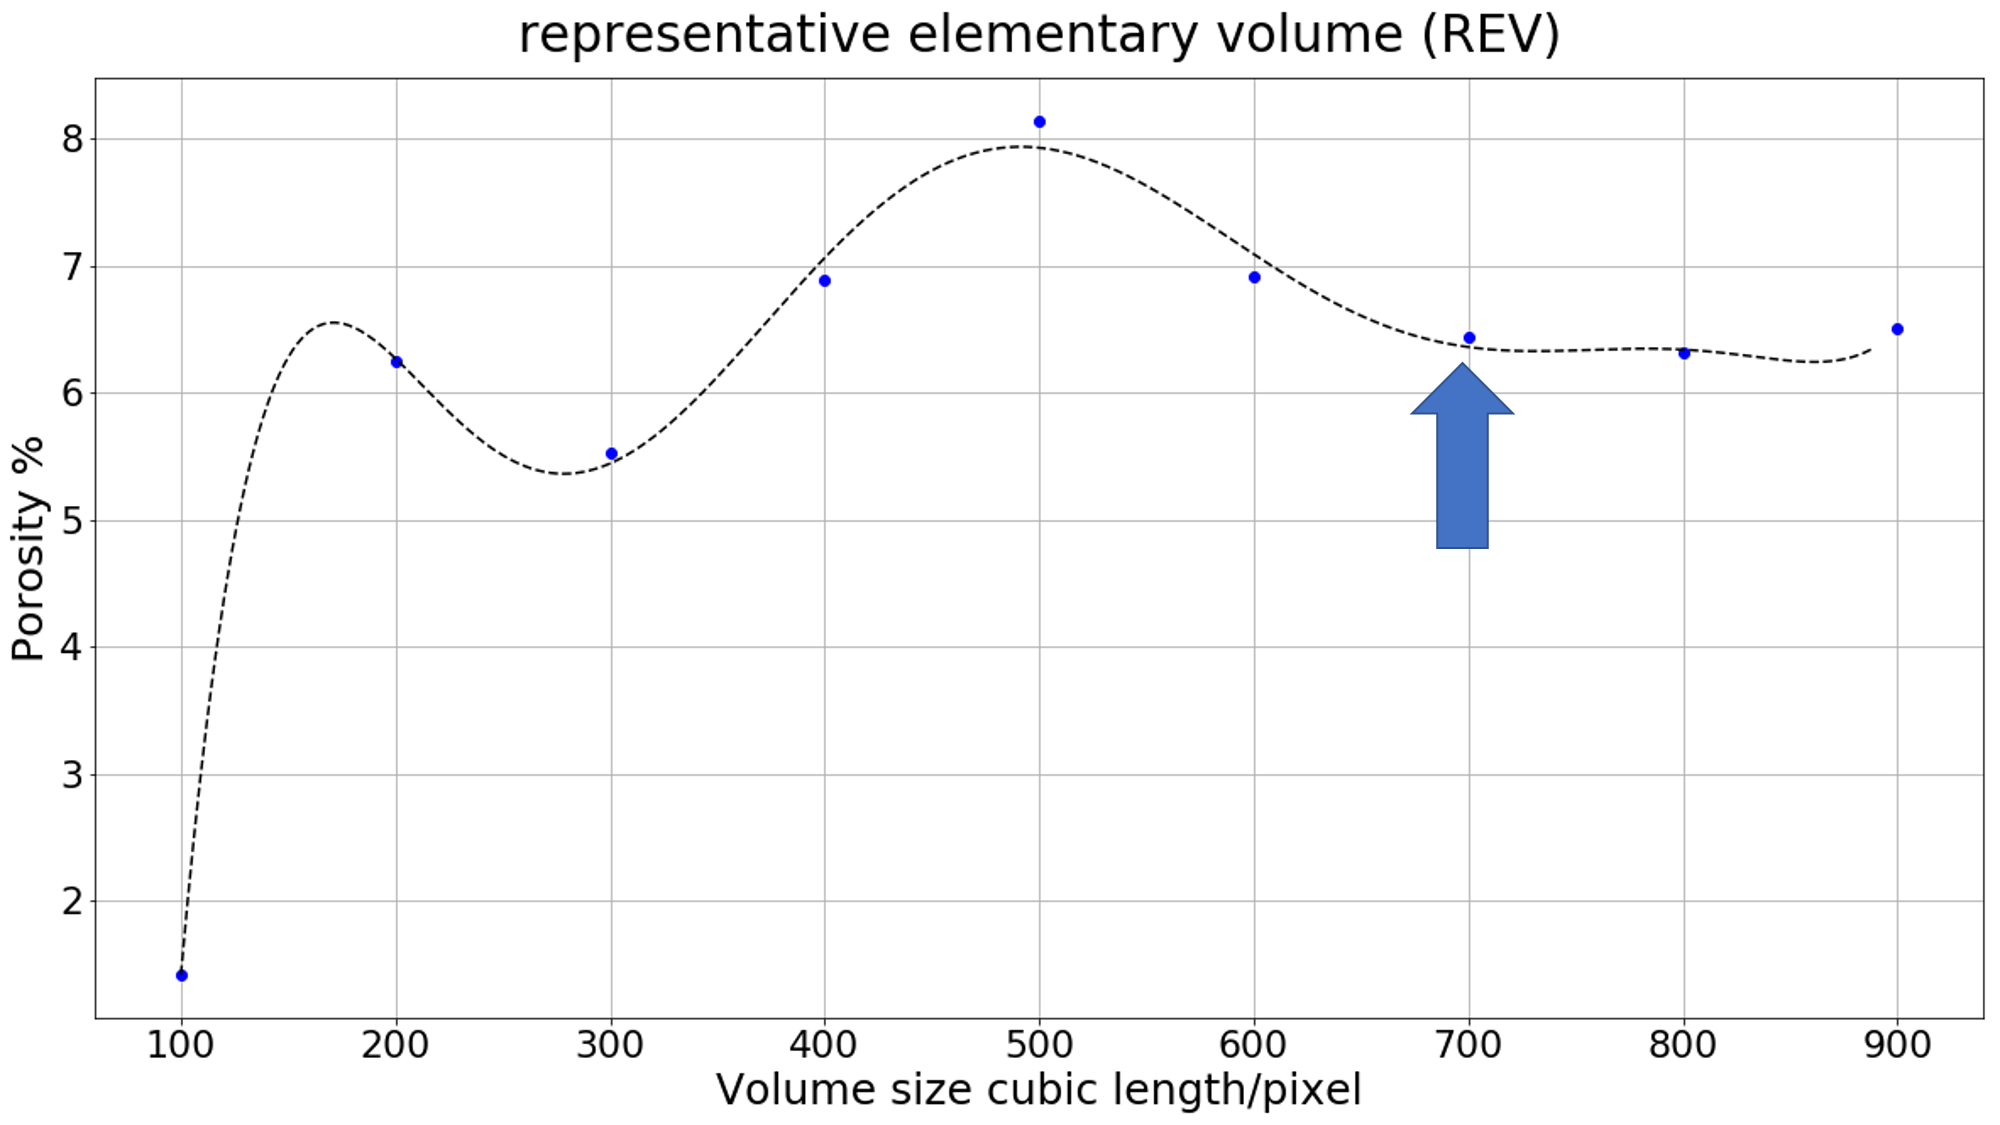
\includegraphics[width=1\textwidth]{\dir/figs/rev.png}
  \caption{The REV curve of targeted volume of Indiana limestone}
  \label{rev}
\end{figure}

\subsection{Wettability}
Understanding wettability of a porous medium (rock formation) is crucial in applications such as contaminant control and enhanced oil recovery.

This Indiana limestone sample has mixed-wettability that large parts of the surface are oil-wet, and also some places especially corners and thinner throats are water wet. Intermediate wet is also found in the pore. Three figures \ref{oilwet},\ref{intermediate},\ref{waterwet} together show the nature of mixed-wettablity of this Indiana limestone. This mixed wettability is presented in both raw CT images and segmentation images. In raw CT images, rock and brine are of similar grey scale, but rock boundary has higher relief and the brine is 'flat' visually, oil was darker grey. In segmented images, rock is labelled black, oil is grey and brine is white. 

In Fig.\ref{oilwet}, five examples of oil-wet surfaces are shown. Contact angles between oil and rock are less than $90^\circ$, and oil shows a convex interface with water that indicating oil-wet surfaces.

\begin{figure}
    \centering
    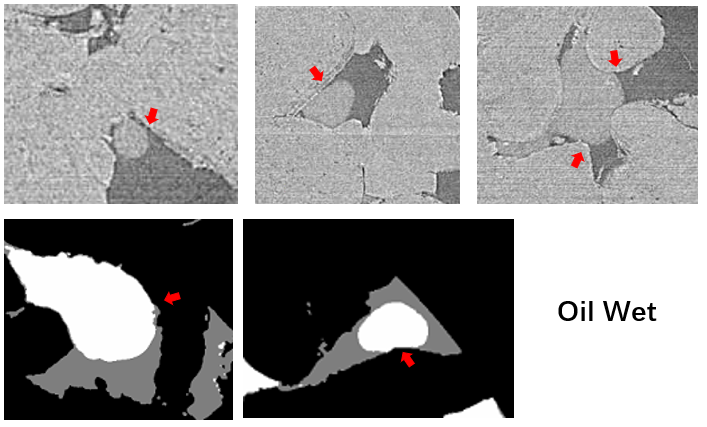
\includegraphics[width=1\textwidth]{\dir/figs/oil-wet.png}
    \caption{Caption}
    \label{oilwet}
\end{figure}

In Fig.\ref{intermediate}, two examples of intermediate-wet surfaces are shown, the contact angles between oil (or water) and rock are near $90^\circ$, indicating intermediate-wet surfaces.

\begin{figure}
    \centering
     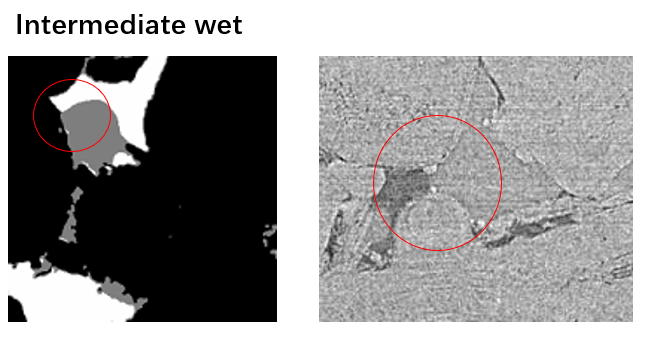
\includegraphics[width=1\textwidth]{\dir/figs/intermediate.png}
         \caption{Caption}
    \label{intermediate}
\end{figure}
     
In Fig.\ref{waterwet}, six examples of water-wet surfaces are shown, the contact angles between oil and rock are larger than $90^\circ$, and oil shows a concave interface with water, indicating water-wet surfaces. A 3D rendering of water-wet pore is shown for visualisation (Fig.\ref{waterwet} bottom). In this pore only oil is rendered and brine is omitted, pore surfaces are rendered transparent. The visualisation shows the convex surfaces of oil blobs in 3D, and the genuine contact angle between oil and rock is larger than $90^\circ$.

\begin{figure}
    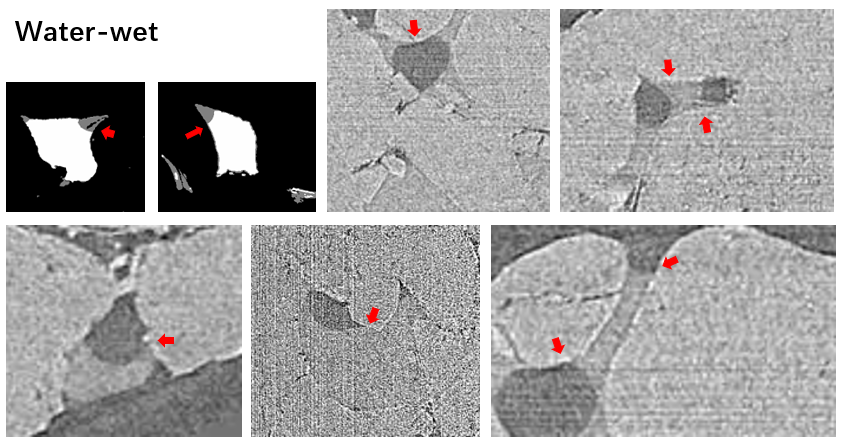
\includegraphics[width=1\textwidth]{\dir/figs/water-wet.png}
    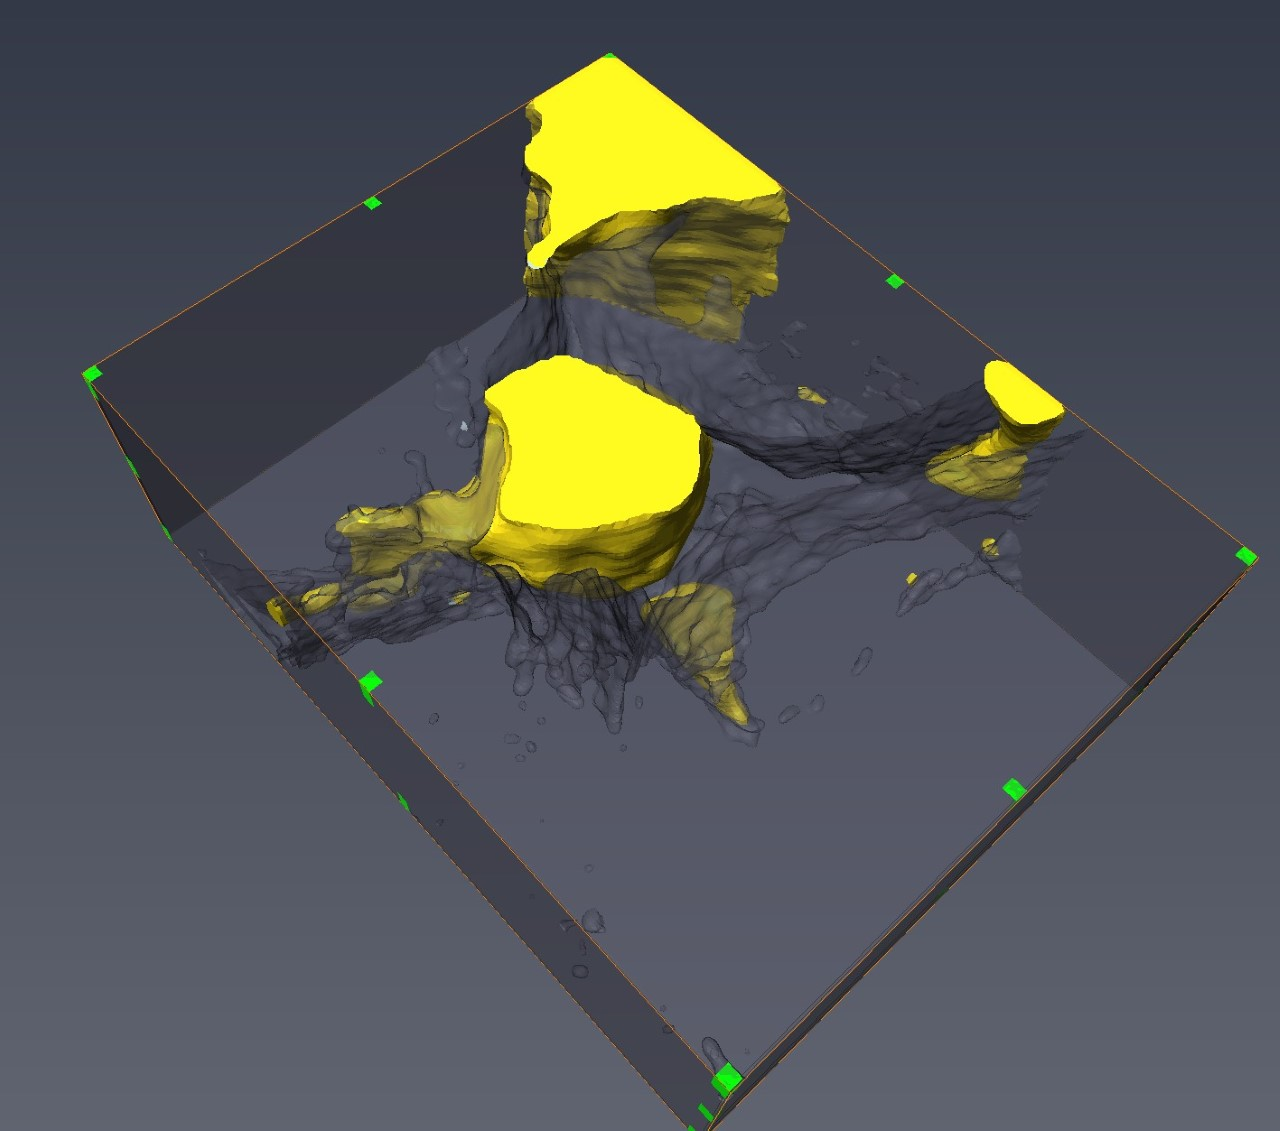
\includegraphics[width=1\textwidth]{\dir/figs/oilblob.jpg}
    \centering
    \caption{Caption}
    \label{waterwet}
\end{figure}

The primary constituents of Indiana limestone is 99\% calcite and 1\% quartz \citep{churcher1991rock}. These minerals are water-wet \citep{abdallah1986fundamentals}, therefore Indiana limestone is normally water-wet prior to oil migration. This studied Indiana limestone sample has unusual wettability that most of the pore surface is intermediate to oil-wet, also parts of the pore surface is water-wet. It was directly from quarry and did not age with oil nor cleaned with solvents. The wettability alteration might be due to highly polar compounds in the impure dodecane. But previous core flooding experiment with the same dodecane \citet{Pak2014thesis} did not develop any oil wet character after even longer exposure. A more likely assumption is that this outcrop Indiana limestone altered its wettability during burial. It is quite possible, especially in shallow environments, for a rock to contact with waters containing dissolved organic acids such as humic acids leached from overlying soil horizons. \citet{blunt2017multiphase} stated that most rocks display some degree of wettability alteration.

\section{Time-resolved imaging and visualisation of fluid displacement process}
X-ray \textmu CT imaging enables in-situ imaging observation of core-flooding process. And image processing and analysis allows quantitative study of the pore structure and fluid flow in the pore space. For example, \citet{ramskill2016fast} imaged the drainage of dodecane in water-saturated Bentheimer sandstone using magnetic resonance imaging (MRI), the results showed the observation of coalescence of discrete non-wetting clusters under time resolution of $\sim 16$ minutes and spatial resolution of ${\sim 0.35} mm/pixel$. \citet{berg2013real} imaged real time 3D Haines jumps of decane-water displacement in a Berea sandstone, under the temporal resolution of 16.8s and spatial resolution of $3\textmu m/pixel$. Results shows that Haines jump as a quantum way of pore filling, typically cascade through 10-20 connected pores, rather than singular pore jump paradigm. \citet{pak2015droplet} imaged mineral oil and KI brine displacement in a Silurian dolomite core using X-ray \textmu CT. The result shows a previously undefined pore-scale mechanism called droplet fragmentation: at high capillary number, trapped non-wetting phase in larger pores can be fragmented into numerous smaller spherical droplets to minimize their surface free energy due to increasing viscous forces. \citet{reynolds2017dynamic} imaged steady state injection of N$_2$ and brine in a Bentheimer sandstone at subsurface reservoir condition, using fast synchrotron X-ray tomography. The analyses show 'dynamic connectivity' of the non-wetting fluid that continuously rearrange between pores like 'traffic light'. These experiments either has low temporal resolution to reveal pore-scale fluid mechanisms of second-scale, or was performed in relatively homogeneous sandstones that limit the variability of capillary forces in the pore system. 

In this experimental study, brine and oil displacement in a highly heterogeneous Indiana limestone was imaged and visualised with the aid of fast synchrotron microtomography. 3D rendering images of the brine is shown in the following subsections.

\subsection{Brine injection}
Brine was injected into oil saturated core at the rate of 2.5 \textmu l/min. The synchrotron X-ray microtomography was able to take 20 CT scans of 1s acquisition at 20 seconds interval. An overall visualisation of fluid displacement process in the core was presented in Fig.\ref{brineinj}. In the figure, Brine is labelled blue and oil is labelled yellow. The orange bounding box shows the field of view (FoV) of the CT scanner. A detailed description of the brine injection will be presented as follow.

\begin{sidewaysfigure}
    \centering
    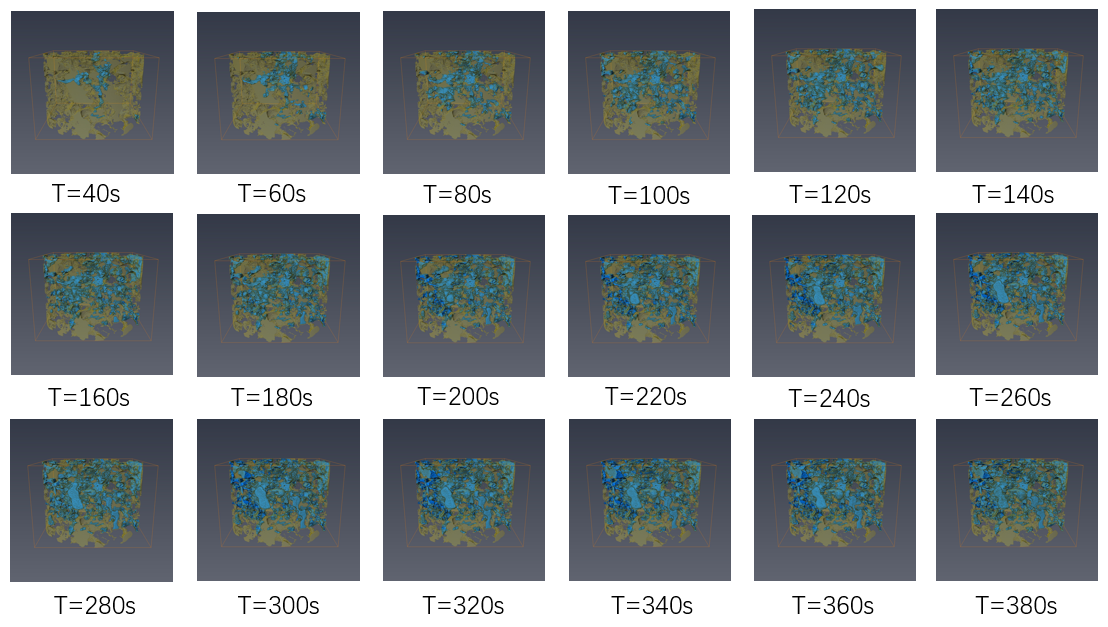
\includegraphics[width=1\textwidth]{\dir/figs/brineinj.png}
    \caption{Caption}
    \label{brineinj}
\end{sidewaysfigure}

The pore space was fully saturated with oil prior to brine injection. At T=40s the CT visualisation shows the first presence of brine in this targeted sub-sample volume (Fig.\ref{1303}). The brine entered the pore space through a single channel and branched in the middle of the core, this bursting of brine pathway happened during the temporal resolution of 20s. This brine cluster was mostly connected except some detachments at the bottom and on the top. A minor blob of brine also entered the volume of interest on the edge. The brine was passing through both narrow throats and larger pores, this observation supports the judgement of a mixed-wet pore system.

\begin{figure}
    \centering
    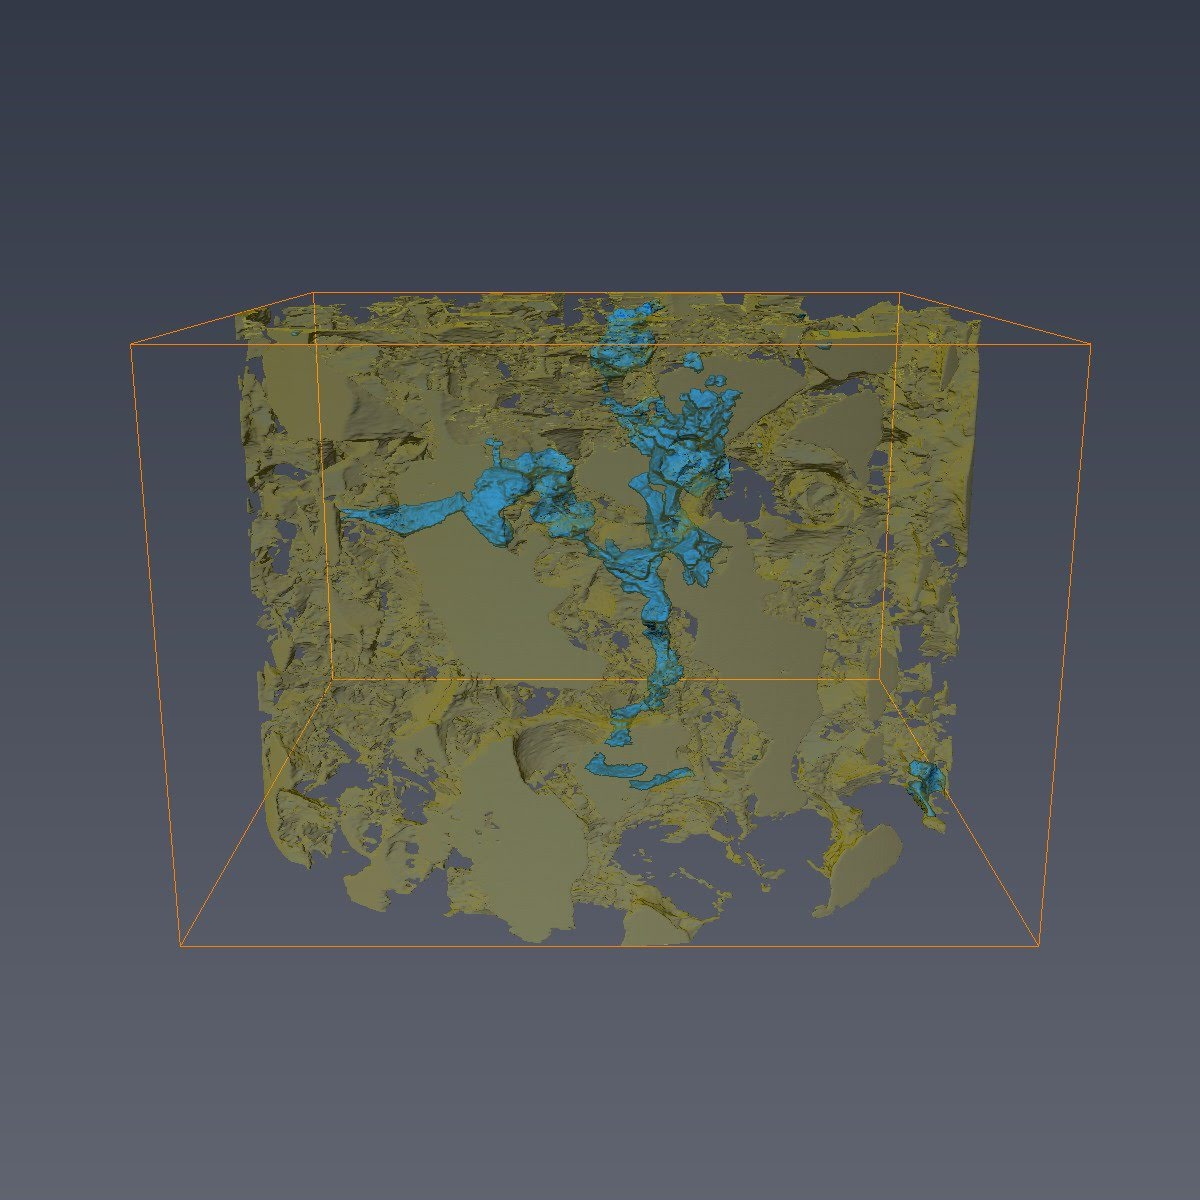
\includegraphics[width=1\textwidth]{\dir/figs/1303.png}
    \caption{Caption}
    \label{1303}
\end{figure}

Fig.\ref{1304} shows the successive CT visualisation of 20s after Fig.\ref{1303} Expansion of the brine were mainly fed by the central pathway established earlier. The small brine blob on the bottom right was also expanded to its adjacent pore. The brine migrated both upwards and laterally through the central pathway. Some brine clusters were disconnected to the main cluster, as the brine injection is mainly a drainage process, the detachment of the clusters was possibly due to Roof-snap off mechanism. At this stage, the displacement processes are fast, we can not observe the on-going drainage process within the temporal resolution of 20s.

\begin{figure}
    \centering
    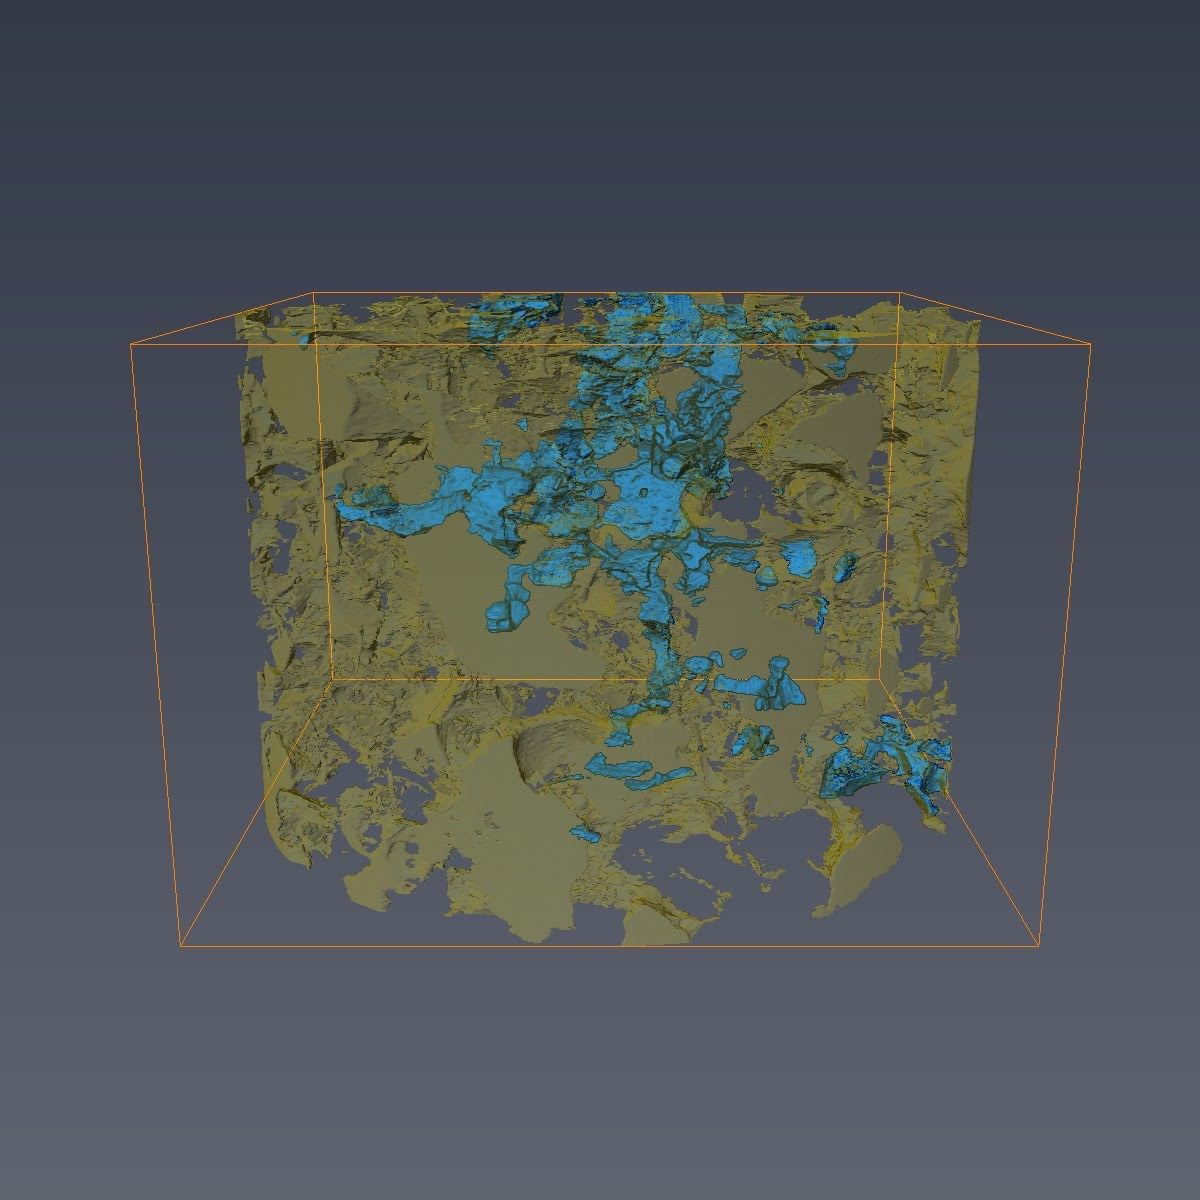
\includegraphics[width=1\textwidth]{\dir/figs/1304.png}
    \caption{Caption}
    \label{1304}
\end{figure}

\subsubsection{Local flow rate variation}
As brine injection continued, the brine clusters kept expanding laterally. But it started to show some variation of local flow rate. Fig.\ref{1305-1312} shows the snapshots of timestamp T=80 to T=220. In this time series, both fast and slow drainage of pores are identified. At T=100s and T=160s, the green arrows point to three clusters that emerged quickly, this could be either a normal drainage process at a faster local flow rate below the CT temporal resolution, or a Haines-jump process. This fast pore filling usually span across multiple pores at one CT scan time step, i.e. within 20s. These fast-growing brine clusters are very similar with Haines-jump observation by \citet{berg2013real} that typically cascade through multiple geometrically defined pores.

For a series of much slower drainage processes, the filling of single bigger pores took 60s or even longer, these slow-filling pores are pointed with red arrows in Fig.\ref{1305-1312}. For these pores, I have the chance to observe on-going drainage process that the brine as non-wetting phase, advanced from the throat to the centre of a bigger pore, and forming a convex interface curvature. 

\begin{figure}
    \centering
    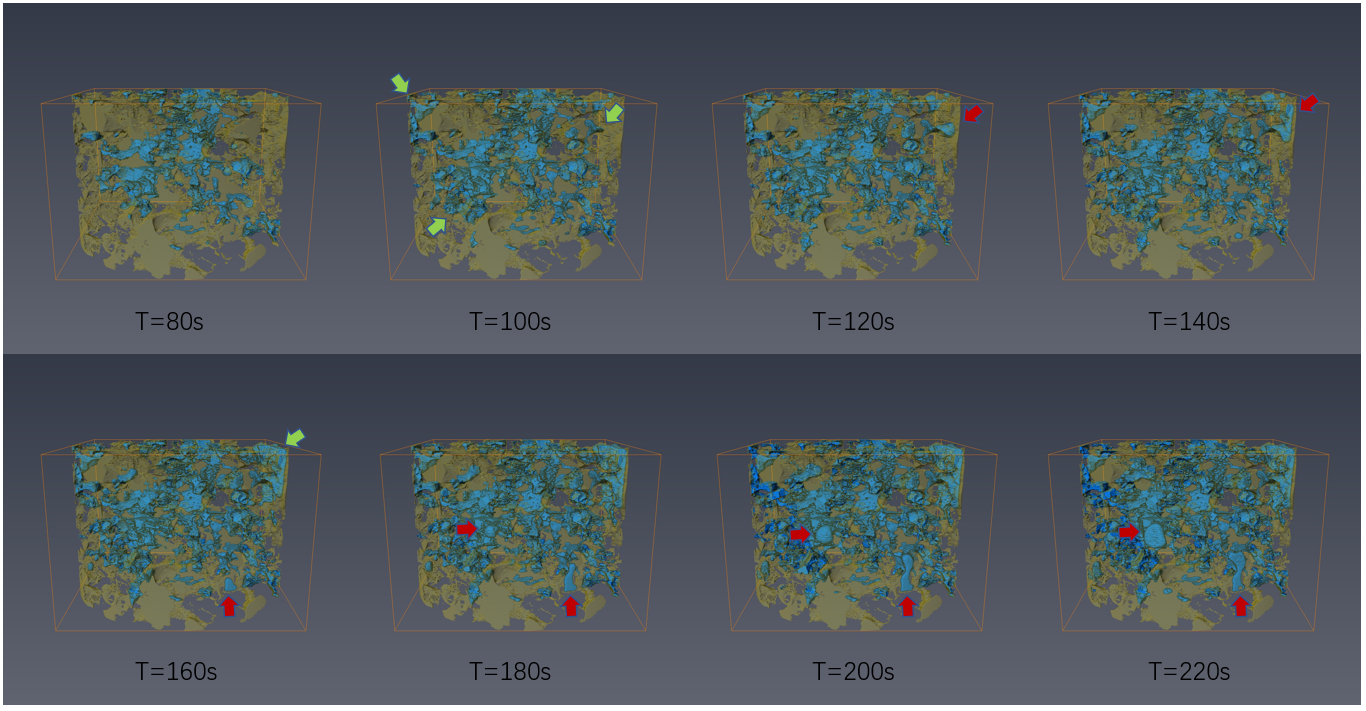
\includegraphics[width=1\textwidth]{\dir/figs/1305-1312}
    \caption{Caption}
    \label{1305-1312}
\end{figure}

Observations shows that the slower drainage can either occur in a single bigger pore, or span across multiple pores. Examples are shown in Fig.\ref{220-360}, in this time sequence, the FoV is zoomed in to show two drainage events masked in red and green. The red cluster was slowly swelling as a single blob in one pore. The green cluster was expanding upwards through three pore throats and filling the pore body smoothly. 

\begin{figure}
    \centering
    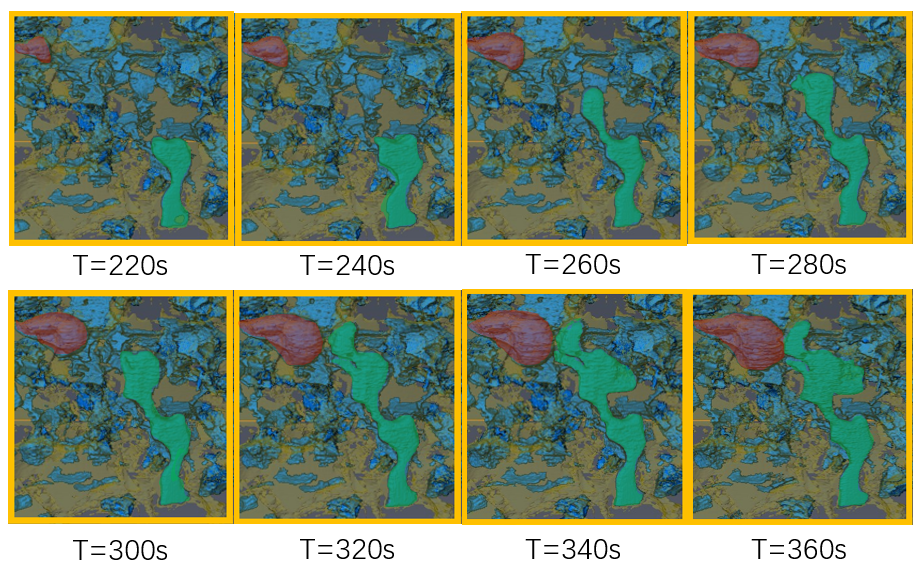
\includegraphics[width=1\textwidth]{\dir/figs/220-360}
    \caption{Caption}
    \label{220-360}
\end{figure}

After one pore volume of brine had been injected, which took around 400 seconds, the brine reached a maximum saturation and the residual oil reached an irreducible saturation. The 3D rendering of the final scan is shown in Fig.\ref{1320} as screenshot. The pores that were not invaded are mainly located at the peripheral or at the bottom plane, either because of insufficient capillary entry pressure, or no accessible route. The brine mainly resides in bigger pores, but also in thin and narrow structures in fewer places. Coalescence of clusters and some local rearrangement of brine blobs are also observed. A link to the video of the complete brine injection process can be found in the appendix.

\begin{figure}
    \centering
    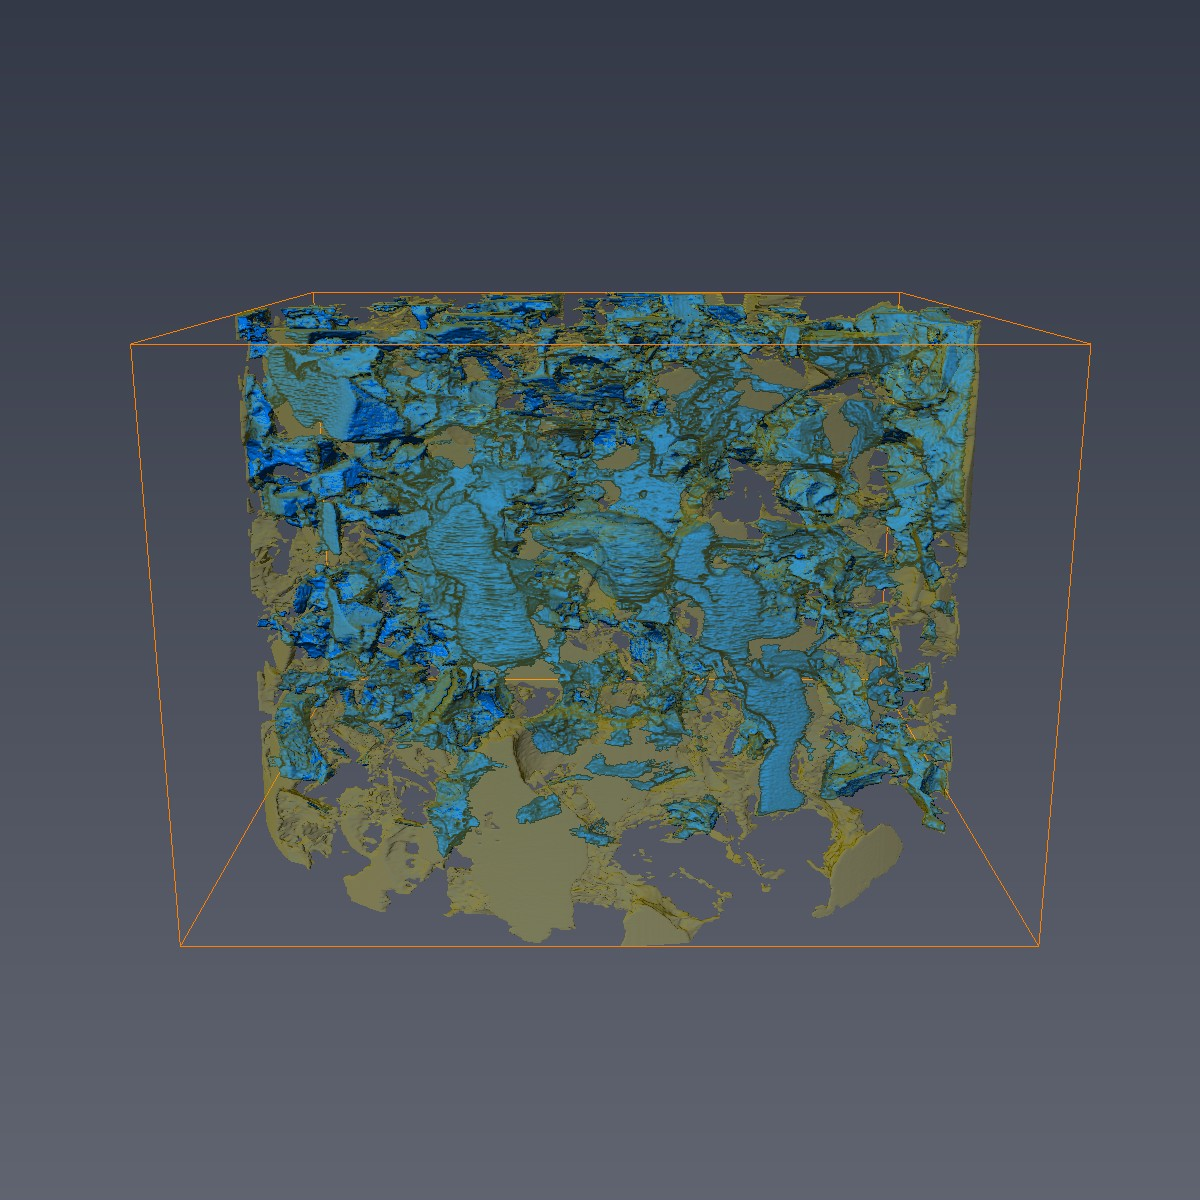
\includegraphics[width=1\textwidth]{\dir/figs/1320}
    \caption{Caption}
    \label{1320}
\end{figure}

\paragraph{Roof snap-off}
During the brine injection which was mainly a drainage process, some snap-off events are identified, and one Roof snap-off (Fig.\ref{roofsnapoff}) has been numerically simulated by our collaborate researcher Dr. Maes, this simulation is described in detail in section \ref{modelling}. 

\begin{figure}
    \centering
    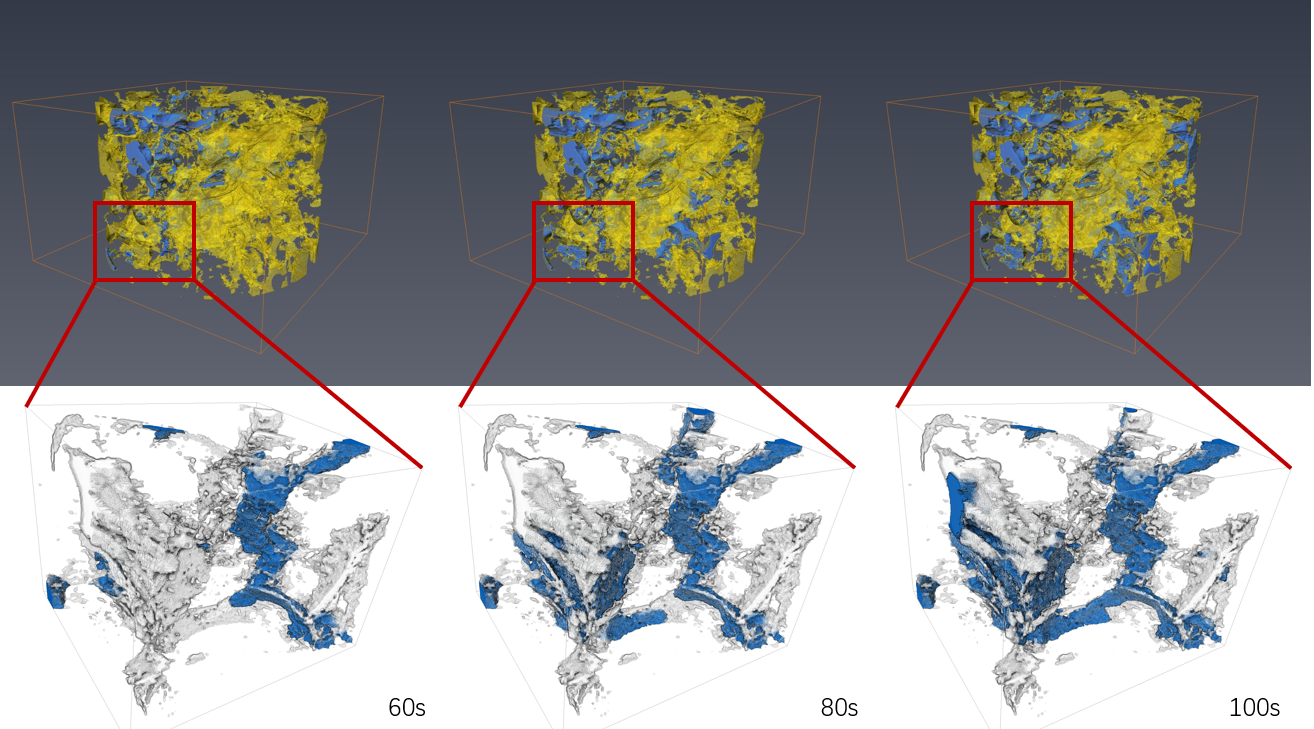
\includegraphics[width=1\textwidth]{\dir/figs/roofsnapoff.png}
    \caption{Caption}   
    \label{roofsnapoff}
\end{figure}

The main events of brine displacing oil has been recorded with twenty CT scans (Exp013). After the main events, the brine injection continued for two more pore volumes. During this continued injection, CT scans showing that the fluid configuration was slightly rearranged, but the analysis shows that the brine and oil saturation had already reached equilibrium at around $brine:oil=53\%:47\%$. In this study we mainly focus on the main displacing events.

\subsection{Oil re-injection}
After the brine injection, oil was re-injected into the core. This is mainly an imbibition process due to the mixed-wet (mainly oil wet) nature of this core. Twenty synchrotron microtomography were scanned and the 3D visualisation is shown in Fig.\ref{oilinj}. The first figure captioned 'Brine saturated' is the last scan before oil entered the core. The first scan at oil re-injection scan T=0s, did not capture the first appearance of the oil, due to the necessary time gap between two batch of twenty scans. This experimental limitation is common in consecutive X-ray CT core flooding experiments, for example \citet{khanamiri2018fluid} also experienced such time gap that caused the failure of capturing the beginning of the injection.

\begin{sidewaysfigure}
    \centering
    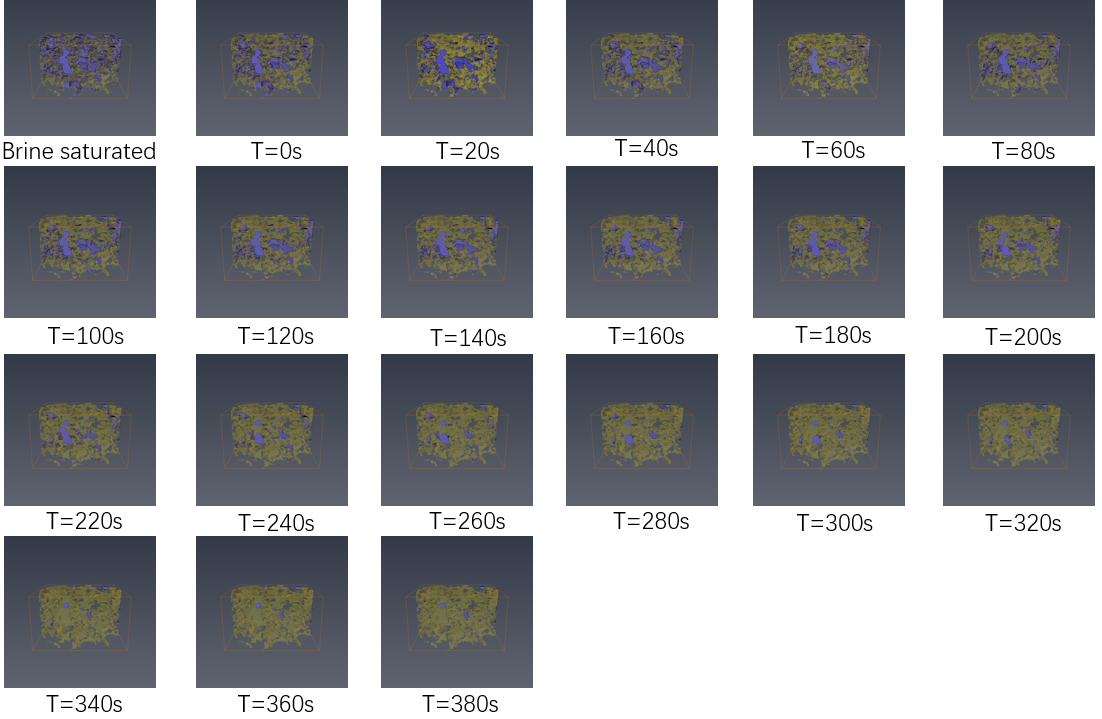
\includegraphics[width=1\textwidth]{\dir/figs/oilinj.png}
    \caption{Caption}
    \label{oilinj}
\end{sidewaysfigure}

At T=0s, the oil has been entering the core for a short period, the image is shown in Fig.\ref{1801}. Part of the brine had already been displaced out of the FoV. The main imbibition processes identified in the oil re-injection are snap-off and piston like advance, the competition of these two processes controls the nature of the displacement \citep{blunt2017multiphase}. The residual brine was fragmented into many disconnected larger clusters, indicating many snap-off events due to the swelling of the oil films during imbibition. Some other pores were entirely displaced, in a piston-like fashion that the advancing water front is rather flat and left no brine trapped.

\begin{figure}
    \centering
    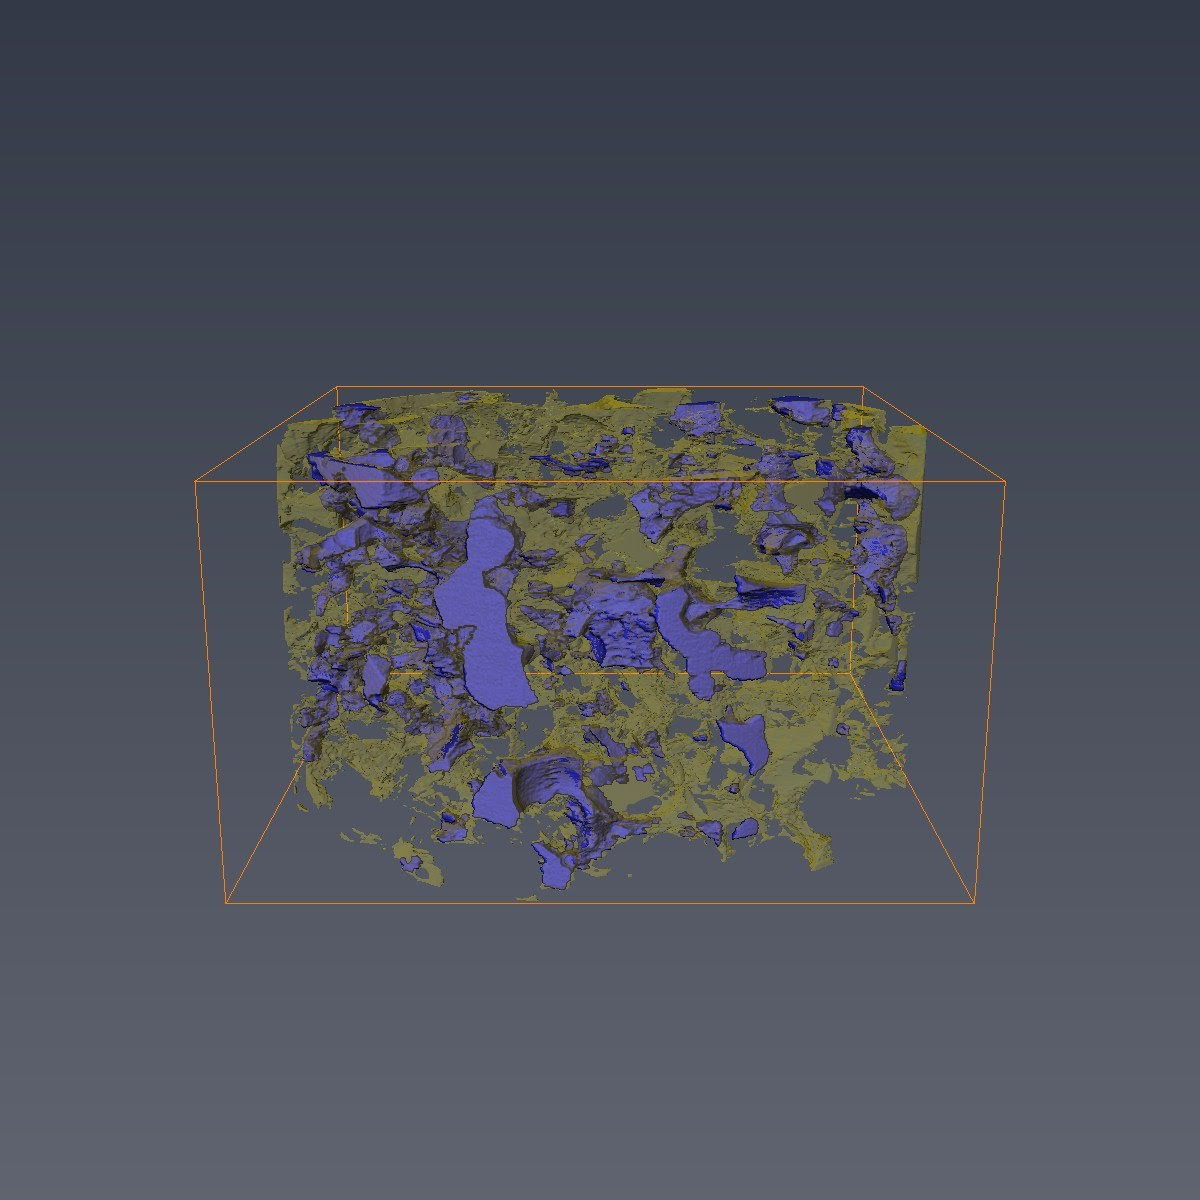
\includegraphics[width=1\textwidth]{\dir/figs/1801}
    \caption{Caption}
    \label{1801}
\end{figure}

\subsubsection{Snap-off}
Two examples of snap-off events are shown in Fig.\ref{snapoff}. The left column shows pre-snap-off clusters that labelled in magenta (red-pink) and cyan (blue-green). These two clusters are snapt-off by the swelling of the oil film during imbibition. The snap-off event happened within 20s and the next scan recorded the post-snap-off of the same clusters (right column). Terminal menisci (TM) were formed after snap-off. The magenta cluster after snap-off formed two TM that curved in two directions, this agrees with the theoretical snap-off paradigm. However the cyan cluster has two unusualness: first the snap-off did not occur at the seemingly narrowest part of the throat; secondly the lower part of the post-snap-off cyan cluster, has a curvature that curved slightly into the same direction with its counterpart. The first unusualness can be explained by a guess that the local arc meniscus (AM) is large, and easier to reach the critical curvature for snap-off to occur, this is possible in this highly irregular pore space in terms of both geometry and wettability. The second unusualness that snapt-off formed two TM that has same direction of curvature, I presume the lower curvature is an unstable curvature that was energetically unfavourable while being imaged, and would quickly shrink to form an curvature that is opposite to its counterpart.

\begin{figure}
    \centering
    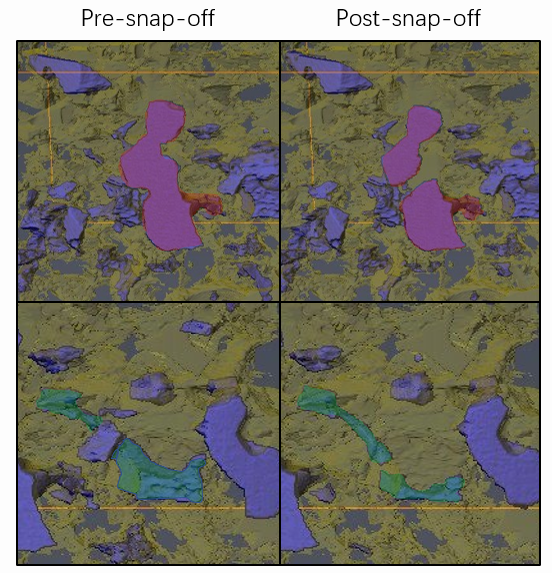
\includegraphics[width=1\textwidth]{\dir/figs/snapoff}
    \caption{Caption}
    \label{snapoff}
\end{figure}

\subsubsection{Piston-like advance}
Another main imbibition mechanism is piston-like advance. An example of observation of on-going piston-like advance is shown in Fig.\ref{pistonlike}. For clearness of visualisation, a rendering of brine clusters that was being displaced by piston-like advance of oil is shown, rather than the advancing oil.

Fig.\ref{pistonlike} shows the time series of a non-wetting brine cluster being displaced by piston-like advance of wetting oil. The cluster in the middle of the images was being displaced, the advancing front is at its right end and pushing towards left. The piston like advance took eight time steps to completely displace the brine cluster in the pore and left no non-wetting phase trapped. This is the reverse of drainage that the TM moves through the throat towards the non-wetting phase.

\begin{figure}
    \centering
    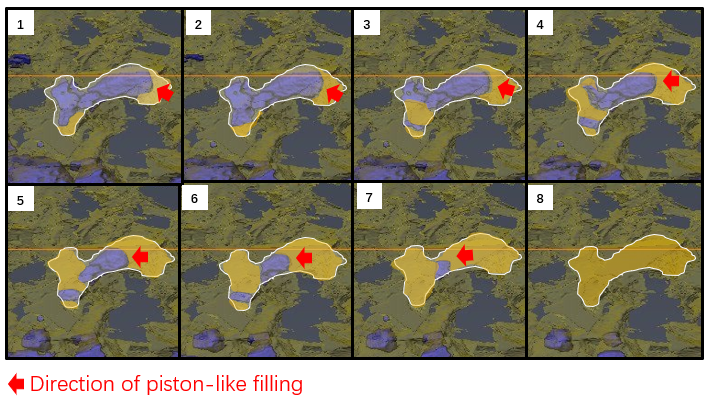
\includegraphics[width=1\textwidth]{\dir/figs/pistonlike}
    \caption{Caption}
    \label{pistonlike}
\end{figure}

\subsubsection{Cooperative pore filling}\label{cooperativeporefilling}
Imbibition is a process that decrease the capillary pressure, so the wetting fluid favours the processes that can reduce more capillary pressure. This means for imbibition it is the pore rather than throats that impedes the filling. To fill a pore in imbibition, the threshold capillary pressure is decided by the maximum radius of the TM curvature of that pore. This curvature is not only dependent on the pore geometry, but also depend on the arrangement of the wetting phase in the bounding throats. 

\citep{lenormand1983mechanisms,lenormand1984role} studied the mechanism that the critical radius of curvature is influenced by the number of bounding throats that filled with non-wetting phase. The mechanism is called $I_n$ where $n$ is the number of throats connected to the pore that filled with non-wetting fluid. For the same pore, the theory states that apart from $I_0$ which is impossible to fill, $I_1$ has smaller critical TM curvature radius than $I_2$. Thus imbibition will prioritise $I_1$ than $I_2$ than $I_3$ and even larger $n$. This eventually lead to a flat frontal advance with no trapping \citet{blunt1992simulation}. 

Cooperative pore filling ($I_1$) is also identified in the studied imbibition process. Fig.\ref{i1} shows an example of $I_1$ type cooperative pore filling. In the highlighted pore, non-wetting brine is labelled blue, and the rest is filled with wetting oil. This is a typical $I_1$ process that only one bounding throat is filled with non-wetting phase. The oil phase in the other two throats was cooperatively displacing the pore-occupy brine. The second figure shows the critical curvature radius of TM for cooperative pore filling to occur. After another two time steps, the non-wetting brine was completely displaced by oil.

\begin{figure}
    \centering
    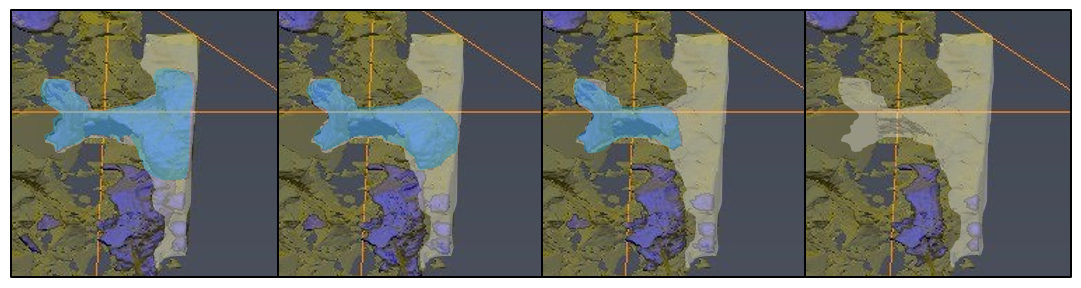
\includegraphics[width=1\textwidth]{\dir/figs/i1}
    \caption{Caption}
    \label{i1}
\end{figure}

\subsubsection{Meniscus curvature fluctuation}\label{meniscuscurvaturefluctuation}
\citep{rucker2015connected} observed successions of snap-off and re-connection events due to fluctuations in local meniscus curvature. They conducted imbibition experiment using CsCl doped water and n-dodecane in a Bentheimer sandstone, and imaged with synchrotron micro CT with frame rate of 40s. The capillary number of water was $1.8\times 10^{-8}$. The Fig.\ref{rucker2015} shows that snap-off events can cause meniscus oscillation, and trigger coalescence of nearby clusters. 

\begin{figure}
    \centering
    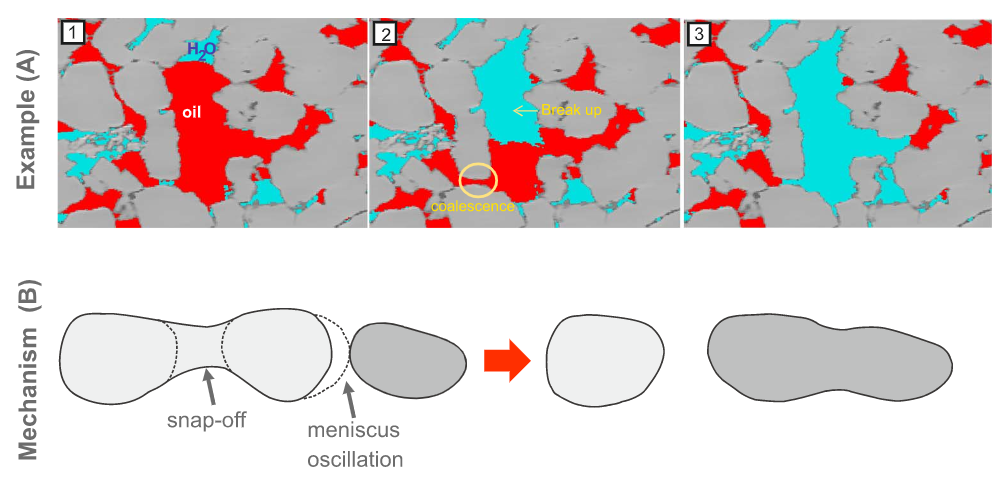
\includegraphics[width=1\textwidth]{\dir/figs/rucker2015}
    \caption{Caption}
    \label{rucker2015}
\end{figure}

Similar phenomenon was identified in this studied imbibition process. The example is shown in Fig.\ref{reconnection}. The snap-off of the upper cluster caused oscillation of the associated meniscus, this oscillation in turn triggered the re-connection of the lower two clusters.

This event is controlled by the ratio of the snap-off threshold pressure to the piston-like advance threshold pressure of the same throat. Theoretically it requires this ratio close to 1 to trigger this process, for which it requires a slit-like throats and contact angle close to zero with little hysteresis \citep{blunt2017multiphase}. However in our observation, the throat for re-connection to occur is not slit-like but is rather wide and short. This can be explained by the rapid pore scale dynamics which lead to a surge in local capillary number\citep{armstrong2013interfacial}, which in turn generated viscous forces that powered the coalescence \citep{rucker2015connected}. This observation underlines the fact that the control of global flow rate and the associated capillary number has limited significance of local pore-scale events.

\begin{figure}
    \centering
    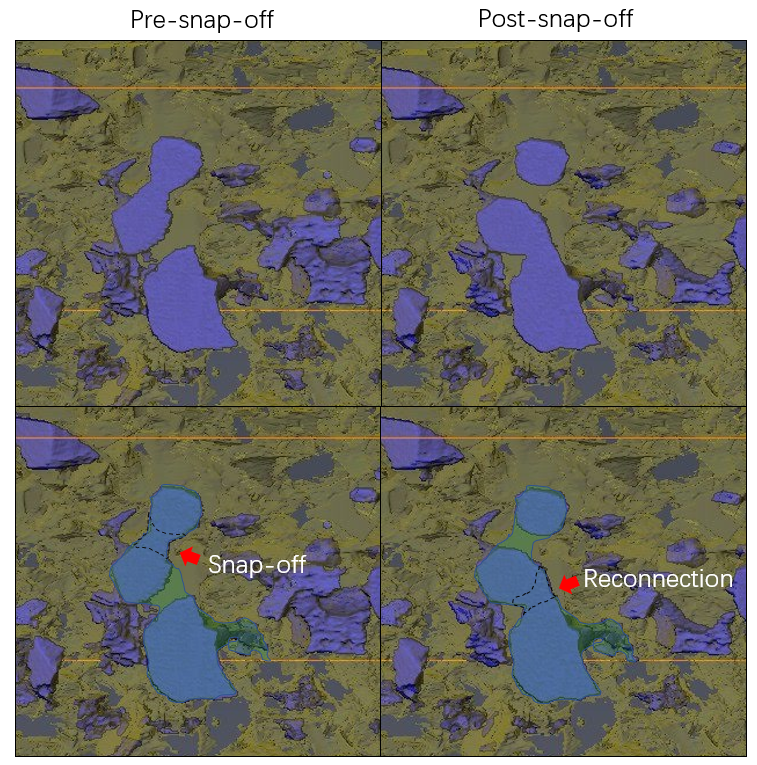
\includegraphics[width=0.7\textwidth]{\dir/figs/reconnection}
    \caption{Caption}
    \label{reconnection}
\end{figure}

 Associating with the former time step in Fig.\ref{snapoff}, this group of brine clusters had experienced a series of dynamic displacement process of wetting layer swelling, snap-off, another snap-off and meniscus oscillation, reconnection and final snap-off. The complete sequence is shown in Fig.\ref{snapoffsequence}. In this figure, time step 1 shows a united cluster that will be further snapt-off into three clusters A, B and C. At time step 2, we see the swelling of the wetting layers due to increased oil pressure. Time step 3 shows the first snap-off event that responding to the wetting layer swelling direction, leading to the detachment of cluster C. The terminal menisci of B and C shrank backwards and formed two opposite curvature to minimise the surface tension. The meniscus on the top of cluster A also shrank to adapt to new capillary equilibrium. Time step 4 shows another snap-off event between cluster A and B occurred immediately after 3. The snap-off event caused meniscus oscillation and triggered the re-connection of cluster B and C, which is very similar with \citet{rucker2015connected}'s finding. Time step 5 and 6 shows the rapid filling of the pore space due to snap-off. This illustrates a series of dynamic displacement processes during imbibition, in a irregular and rather large pore space. The displacement processes occurred in a time total of around 120 seconds.
 
\begin{figure}
    \centering
    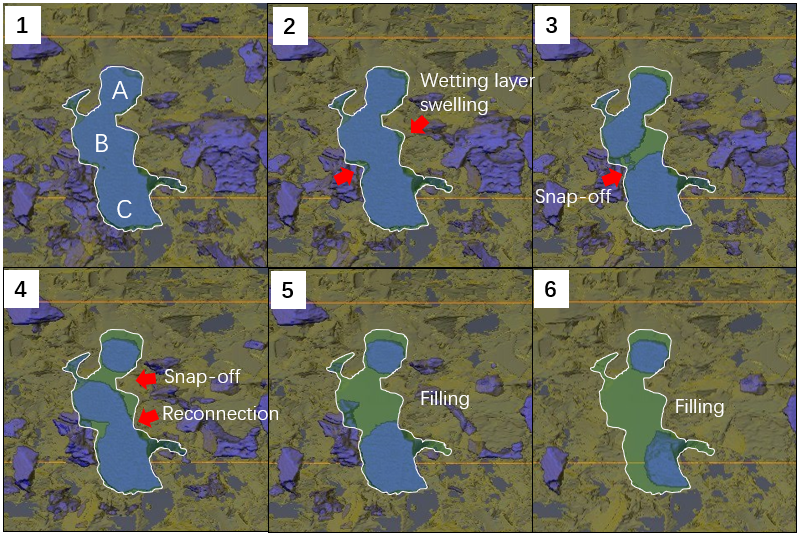
\includegraphics[width=1\textwidth]{\dir/figs/snapoffsequence}
    \caption{Caption}
    \label{snapoffsequence}
\end{figure}

\subsubsection{Trapping}
The clusters that surrounded by snapt-off throats were eventually trapped. Fig.\ref{1820} shows the trapped brine clusters that became immobilised at the end of oil re-injection. The saturation of trapped non-wetting phase, called irreducible saturation, is below 1\% in the studied volume. This indicates that the piston-like advance events are overtaking the snap-off events by a great amount in this pore system. After the main displacement stage, two more pore volumes of oil were further injected to ensure the residual brine reached irreducible saturation.

\begin{figure}
    \centering
    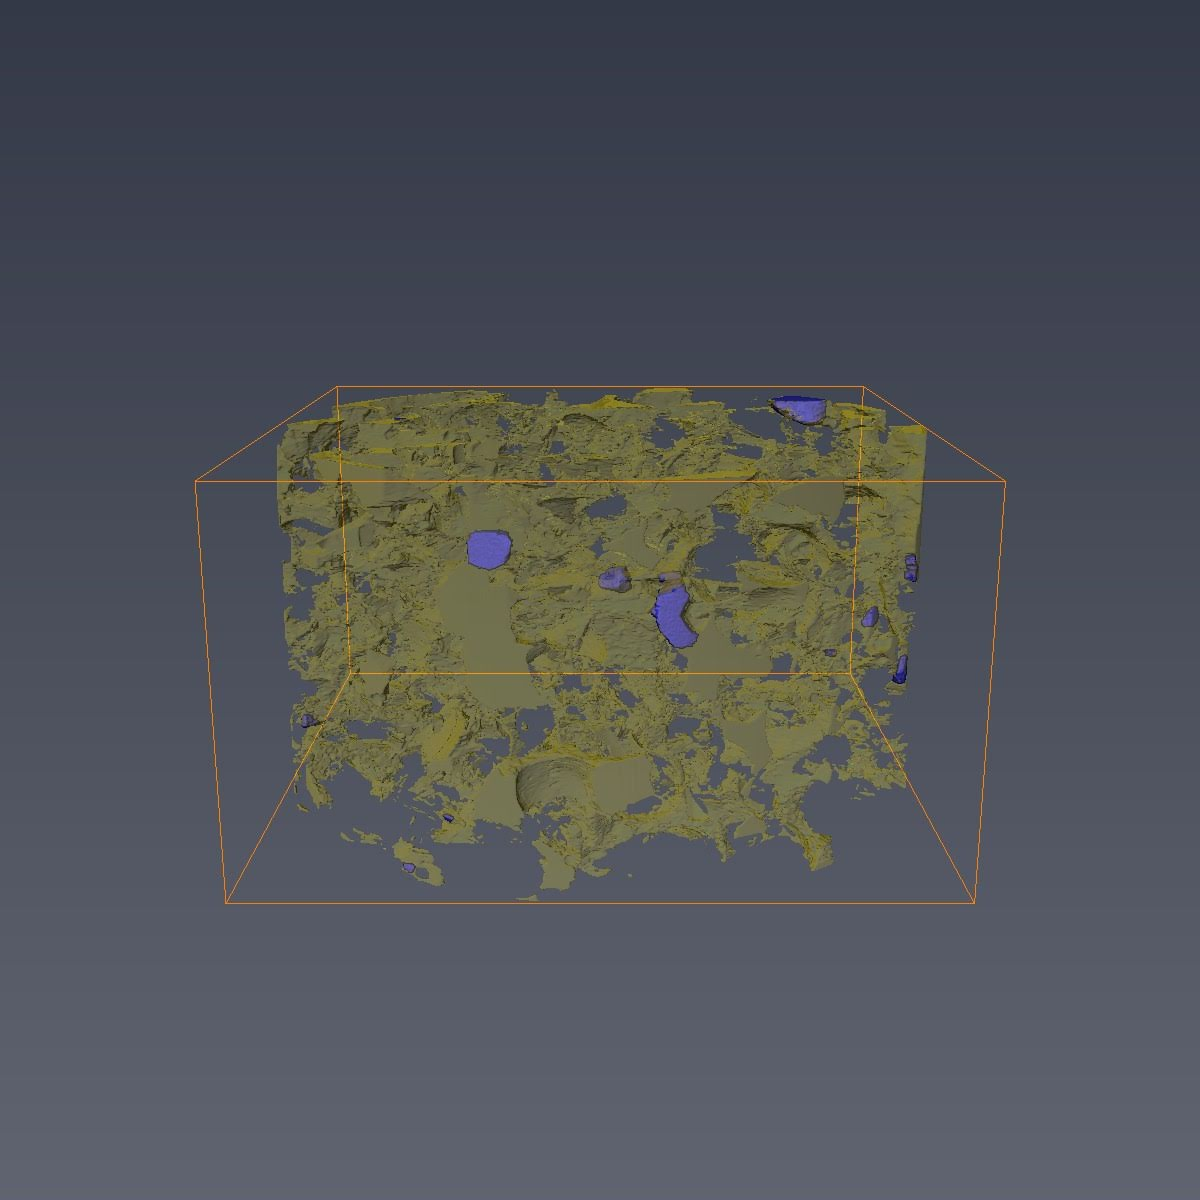
\includegraphics[width=0.7\textwidth]{\dir/figs/1820}
    \caption{Caption}
    \label{1820}
\end{figure}


\subsection{Oil-brine steady state injection}
Steady-state injection of both oil and brine were performed after oil re-injection. The main injection stage took a total of 1060s, during which 53 CT scan volumes were recorded. The injection followed immediately after the end of oil re-injection where the residual irreducible brine saturation is below 1\%. Fig.\ref{ss1,ss2,ss3} shows the visualisation of the complete steady-state injection. In these visualisation, only brine clusters were rendered in 3D to maintain a clean view. It is assumed that the rest of the pore space is fully saturated with oil.

\begin{sidewaysfigure}
    \centering
    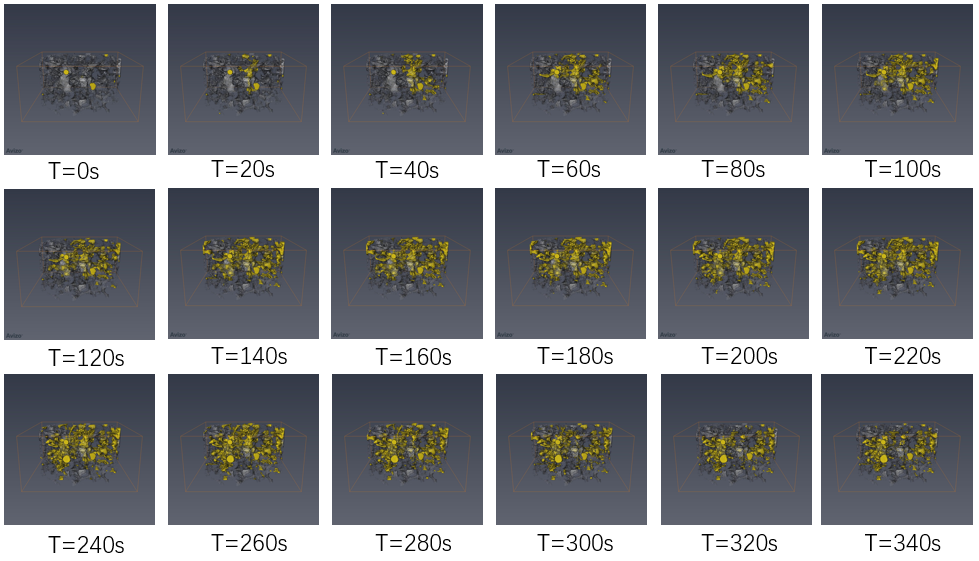
\includegraphics[width=0.9\textwidth]{\dir/figs/ss1.png}
    \caption{Caption}
    \label{ss1}
\end{sidewaysfigure}

\begin{sidewaysfigure}
    \centering
    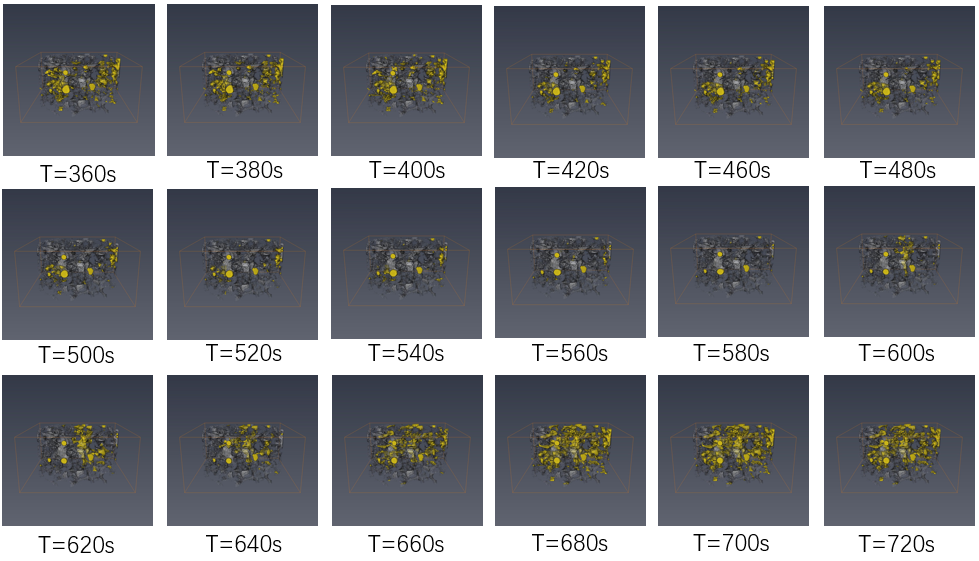
\includegraphics[width=0.9\textwidth]{\dir/figs/ss2.png}
    \caption{Caption}
    \label{ss2}
\end{sidewaysfigure}

\begin{sidewaysfigure}
    \centering
    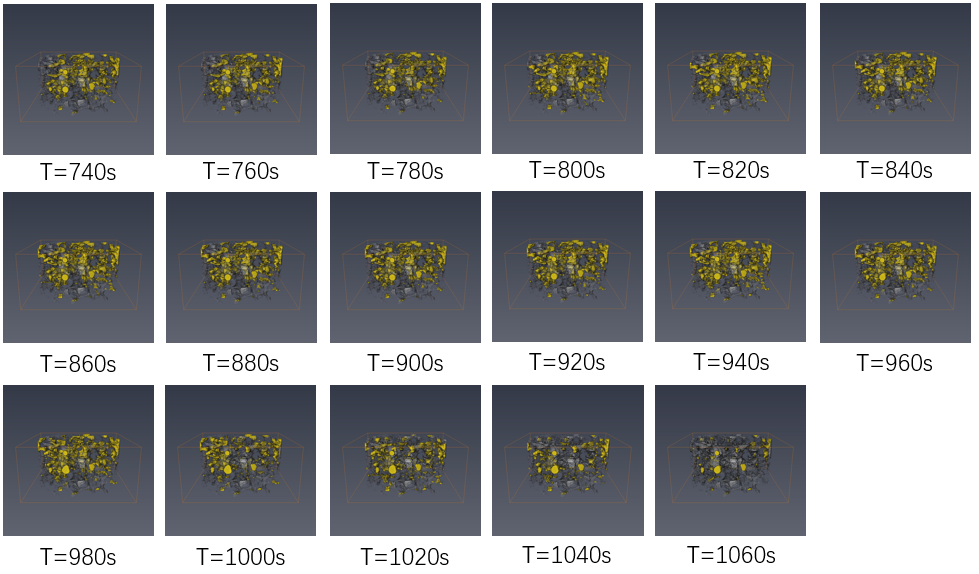
\includegraphics[width=0.9\textwidth]{\dir/figs/ss3.png}
    \caption{Caption}
    \label{ss3}
\end{sidewaysfigure}

\subsubsection{Central fluid channel}
The early stage of steady state injection behaved similarly with the brine injection that both were forming a central fluid channel of brine pathway that penetrated the whole volume of interest. The difference is that in steady state injection no brine was branched laterally. The central fluid channel that acts as feeder channel for both wetting and non-wetting fluids is shown in Fig.\ref{centralchannel}, pointed with red arrow. Fig.\ref{centralchannel} upper row shows in steady-state injection, brine as the non-wetting fluid displace the oil in the central fluid channel firstly. The bottom row shows oil as the wetting fluid uses the same channel too during imbibition. This demonstrates that the access of both fluids are mainly controlled by this single channel. Although oil and water have different preference on the throat radius when they approach the inlet face, it seems that this lack of choice on the inlet face forced the entrance of oil and brine using the same channel. Although other entries do exist on the inlet face, this central fluid channel dominates the fluid entrance of this volume.

\begin{figure}
    \centering
    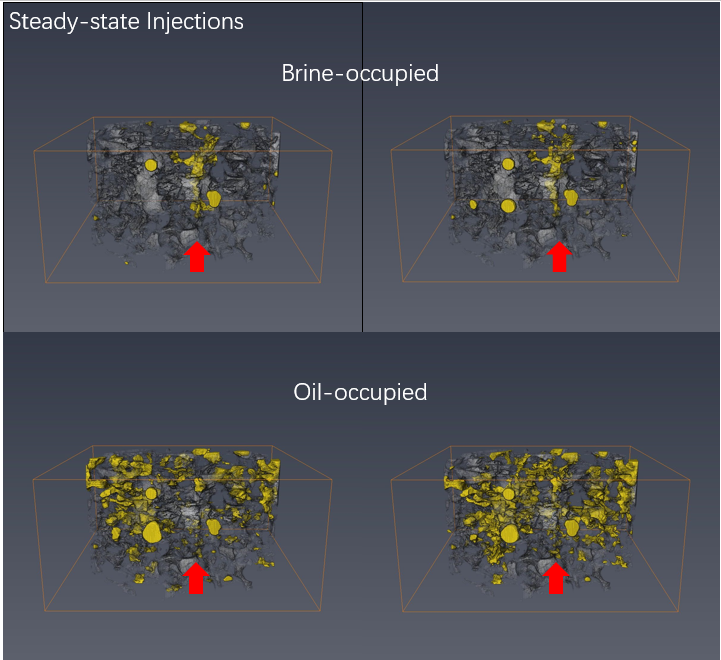
\includegraphics[width=1\textwidth]{\dir/figs/ss_bi_compare1}
    \caption{Caption}
    \label{centralchannel}
\end{figure}

\subsubsection{Emulsion formation and trapping}\label{emulsionformationandtrapping}
\citet{pak2015droplet} observed emulsion formation at high capillary number in a pore with large aspect ratio due to droplet fragmentation. In this study we observed emulsion formation at low capillary number, steady-state injection in pore throat, and ultimately led to emulsion trapping in the pore body.

Fig.\ref{emulsion} shows the process of emulsion formation and trapping. Figure 1 shows the location of pre-emulsion formation at the pore throat. In figure 2, the previously oil-occupied throat was displaced by brine, and emulsion of small brine droplets started forming. At this stage the emulsion had not been completely formed and the small droplets were still partly attached to the brine cluster. In figure 3 we see emulsion of brine reshaped as spherical to minimise the surface energy, they arranged as an alignment which restrained by the elongated throat. And the terminal meniscus of brine had been retreated to the throat entrance. In figure 4 the smaller emulsion droplets coalesce into different sizes and still resided in the throat. In figure 5 one bigger emulsion droplet travelled into the wider pore body, and started splitting into two smaller droplets. Figure 6-10 shows the imbibition of oil in the pore system displaced the connected brine clusters and also brought some emulsion droplets away. But the two droplets in the pore was eventually trapped.

The whole process was very dynamic and had not been previously observed. This may be explained by the opposite flow directions of two fluid phases in the same throat powered by steady-state injection, which led to a surge of relative flow rate therefore higher capillary number. With the fact that local flow rate can be much higher than the global injection rate due to dynamic pore scale events like Haines-jumps \citep{armstrong2013interfacial}, fluid regime can switch from capillary regime to viscous regime and allow the emulsion formation.

The emulsion formation in this pore is not serendipitous, but a constant event that has been observed multiple times during the steady-state injection period. As the pore frequently switched the fluid occupancy, brine emulsion had been formed and merged for multiple times.

One fact that must be point out is that the 'wall' on the right side of the pore, is the heat shrink sleeve that bounding the core perimeter, which may have different wettability than the rock. This may have limited influence on the local flow behaviour, nonetheless, the observation of emulsion formation and trapping is genuine.

\begin{figure}
    \centering
    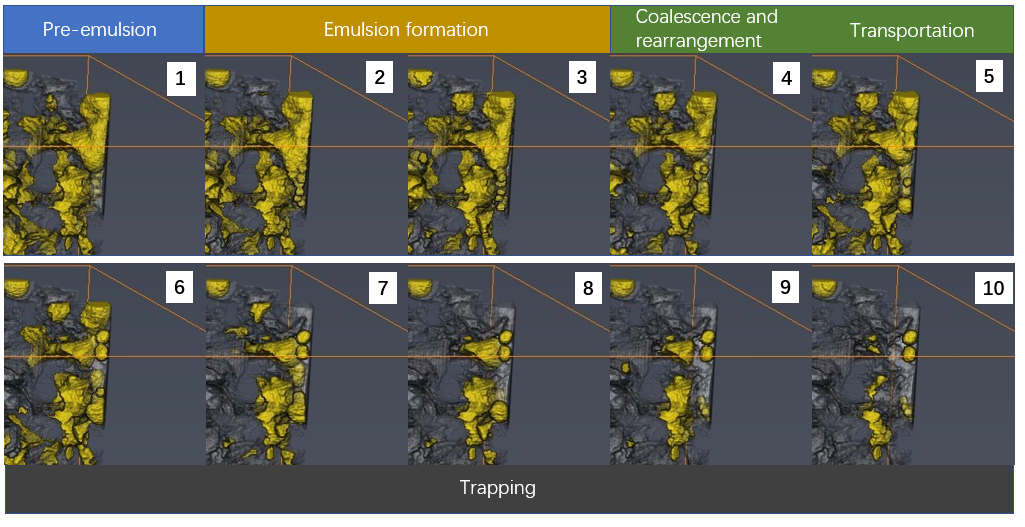
\includegraphics[width=1.1\textwidth]{\dir/figs/emulsion}
    \caption{Caption}
    \label{emulsion}
\end{figure}

\section{Fluid saturation tracking}
Fluid saturation and distribution during displacement has been extensively studied experimentally, as this is closely related to residual hydrocarbon saturation in petroleum industry. \citet{prodanovic20073d} studied the residual oil and water before and after aqueous gel injection in a Berea sandstone, and imaged with X-ray tomography. They analysis shows the residual brine and oil distributions in different pore and throat sizes are not strongly correlated with the effect of gelation. \citet{shi2011supercritical} studied core flooding of supercritical CO$_2$ and CO$_2$ saturated brine in a Berea sandstone (10MPa, 40$^\circ$C), and imaged quasi-static with X-ray microtomography, and a 1D model was made to history-match the saturation profile evolution.  \citet{iglauer2012comparison} studied residual oil saturation of brine-decane flooding in a crude-aged Clashach sandstone and an analogue water-wet sandstone, and imaged with \textmu CT. The results shows that the residual oil cluster size distribution is consistent with the percolation theory, and the residual oil clusters have fewer larger clusters in the oil-wet case than in the water-wet case. In this study, the saturation of two fluid phases during drainage, imbibition and steady steate injection were both monitored with high temporal resolution \textmu CT imaging.

Fig.\ref{satuall} shows the overall brine saturation evolution during brine injection (BI), oil re-injection (OR) and steady state (SS) injection. The six vertical blue lines in the figure separate the saturation curve into seven sections, each section is a batch of 20 CT scans acquisition and labelled with a cartoon indicating the injection status (BI, OR and SS). The core was fully saturated (100\%) with oil prior to experimental injections. During brine injection (t=0-800s), the initial oil was displaced by the invading brine to an irreducible saturation above 40\%. After oil and brine saturation reached equilibrium, oil was re-injected into the core. The residual brine was displaced by the invading oil and almost swiped out all residual brine. Steady state injection of both brine and oil was then performed. A cyclic saturation curve shows the brine saturation during steady state injection. Brine quickly reached 40\% saturation at the onset of injection, then started to decrease showing that oil flow started to dominate. As soon as the saturation of brine reached near-zero, brine flow switched back to domination, the saturation of brine raised again with similar rate as in the beginning. The saturation reached near 40\% and fluctuated for $\pm 5\%$ lasted for around 300 seconds, and eventually hit 40\% saturation. Similar with the first cycle, the brine saturation plunged to zero again after it reached 40\% saturation. The injection was ceased at 2800s, during which 140 CT volumes were taken. One thing to be noted is that the 2800s of experiment is not seamless recorded. The camera had to dump data every 20 scans (400 seconds), which took few minutes. So every 400s a blue vertical line is drawn on Fig.\ref{satuall}, indicating the camera-down time between each batch of scans. 


\begin{figure}
    \centering
    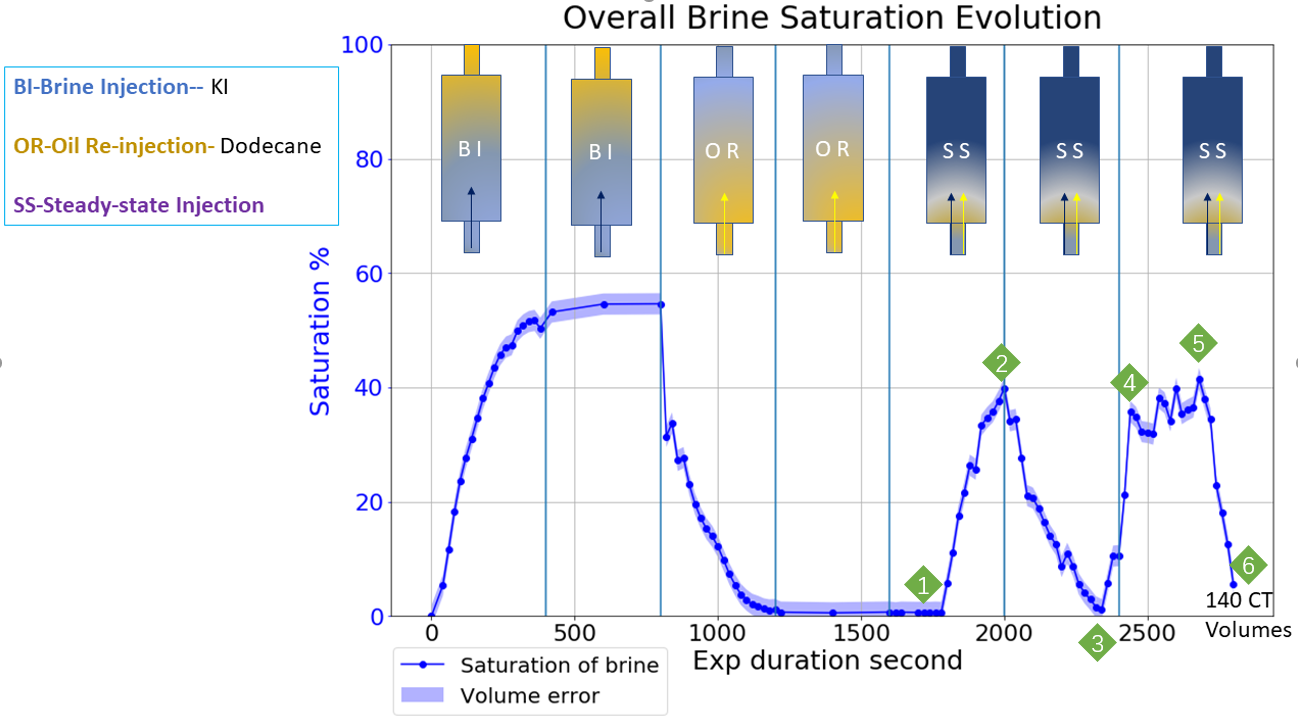
\includegraphics[width=1\textwidth]{\dir/figs/satu_all.png}
    \caption{Caption}
    \label{satuall}
\end{figure}

\subsection{Saturation in drainage and imbibition}  
\subsubsection{Drainage}
The fluid injection began with brine injection into oil saturated core. Fig.\ref{satu1} shows the residual fluid saturation of both brine and oil during brine injection. The oil was steadily displaced by brine, and the saturation for both fluids gradually reached equilibrium after more than 60\% pore volume of brine injected. This shows brine, as the non-wetting phase for the most part of the pore space, filled larger pores at the beginning because of lower capillary entry pressure. As the larger pores gradually saturated with brine, smaller adjacent pores were filled subsequently until the brine inlet can not accumulate enough pressure to overcome the capillary entry pressure of the rest of the pores. Equilibrium was then reached and further injection would not reduce the residual oil saturation.

\begin{figure}
    \centering
    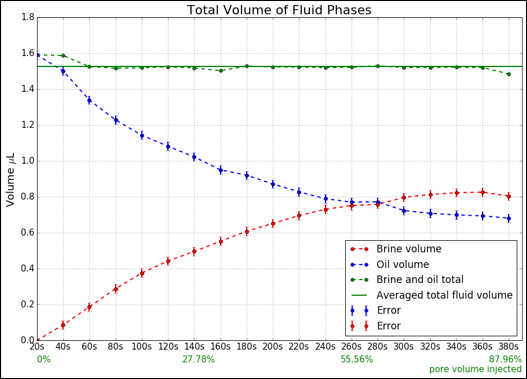
\includegraphics[width=1\textwidth]{\dir/figs/saturation1.png}
    \caption{Caption}
    \label{satu1}
\end{figure}

Fig.\ref{satu1} shows the bulk saturation evolution during brine injection. But it does not tell the saturation distribution inside the highly heterogeneous carbonate rock. To illustrate the saturation distribution along different position in the vertical axis of the core, the injected brine saturation profile along the core is plotted in colour from black to light blue representing injection time from t=60s to t=400s. The core vertical saturation profile is shown in Fig.\ref{brinesatu}. The saturation curves indirectly show the distinctive pore geometry along the vertical axis of the core. The wider a particular colour in the plot, indicating the more saturation increment in a single scan period (20s). In the middle of the core ($distance = 500$) there is a distinctive 'barrier' separating the lower half and upper half of the core. For the lower part of the core ($distance < 500$), the early injection stages from 60s to 160s contributed the majority of the brine saturation, the saturation was less increased in the further injection. The saturation increment of the upper half core, however, was more evenly increased. This difference in brine saturation is due to varied pore size distribution, the lower part has more larger pores which are preferred for the non-wetting brine phase, because this rock is largely oil-wet. As soon as these larger pores were filled quickly in the beginning, the smaller pores were unfavourable for the brine to invade, but instead the intermediate-sized pores in the upper half of the core was filled steadily.

\begin{figure}
    \centering
    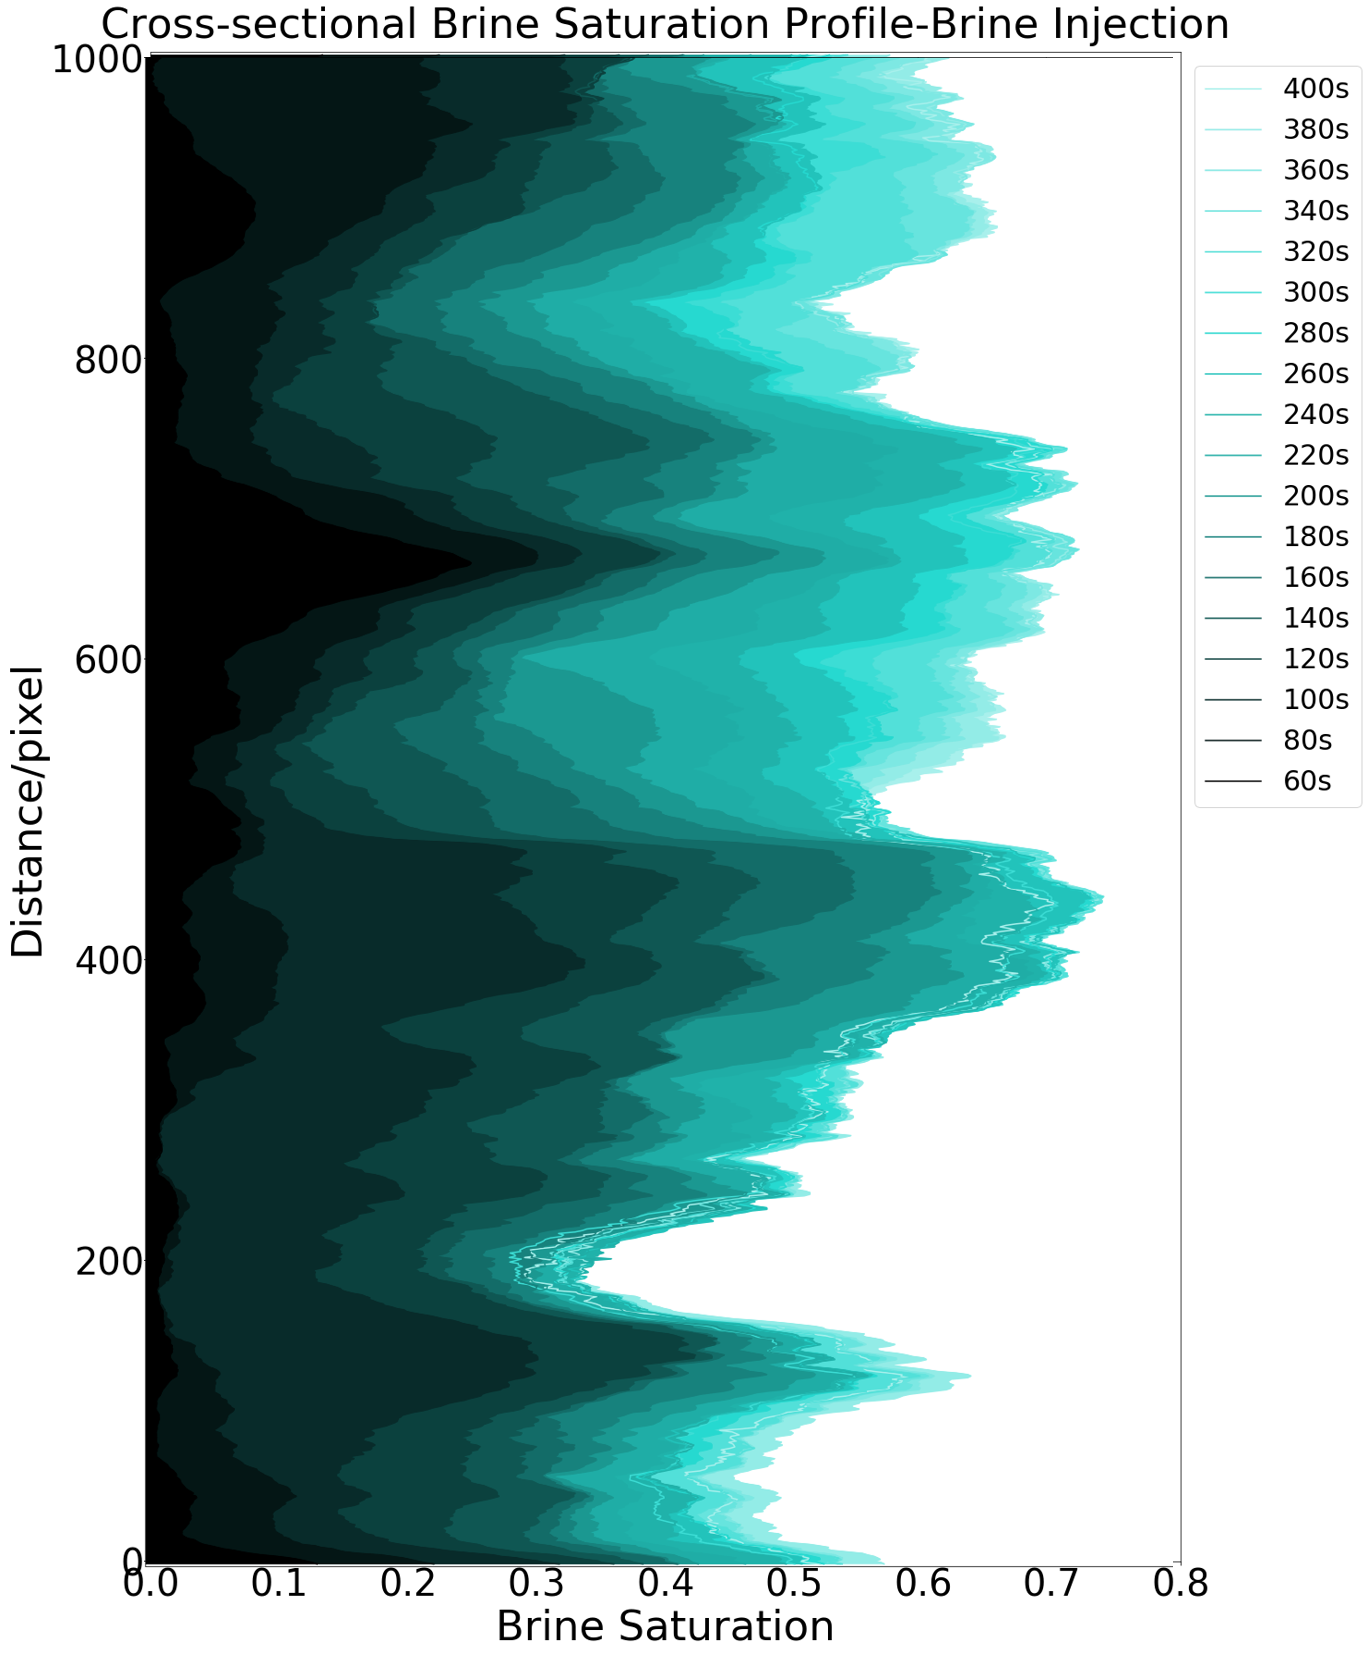
\includegraphics[width=1\textwidth]{\dir/figs/brine_satu.png}
    \caption{Caption}
    \label{brinesatu}
\end{figure}

\subsubsection{Imbibition}
Similarly as Fig.\ref{brinesatu}, Fig.\ref{oilsatu} shows the brine saturation profile during oil re-injection. There are two batch of CT scans recording the oil re-injection stage, the saturation of the first batch is plotted in green tones, and blue tones for the second batch. There was a time gap between two batches of CT scans because of the time needed for transferring data. Therefore the record of fluids saturation between the two batches of CT scans were uncaptured for few minutes, this gap is shown on the figure as the wide area of light green between blue curves and green curves. This time gap is also shown on Fig.\ref{satu1} vertical blue line at t=800. At the beginning of the oil re-injection, the core was partially filled with brine, the saturation profile at the beginning does not match the saturation profile at the end of brine injection because another imaging gap was at the end of the brine injection. This time gap is also shown on Fig.\ref{satu1} vertical blue line at t=400. The t=20s of oil injection is corresponding to overall time t=420s on Fig.\ref{satu1}.

The displacement of brine by the invading oil is shown on Fig.\ref{oilsatu}. The brine saturation was steadily reduced, and the displacement rate varied along the vertical axis of the core. At the onset of oil re-injection, the residual brine distribution in the core was that the upper half has slightly more brine, but more evenly distributed than the lower half. At t=20s-400s the brine saturation was stable, because the injected oil had not reached the bottom of the core yet, the inlet was still brine. The saturation of brine only fluctuated at a very small range due to some minor rearrangement in place. The oil actually entered the core slightly earlier than t=420s, but due to the camera-down time and the temporal resolution of the X-ray tomography, t=420s was the first scan of oil re-entering the core. As the oil re-injection went on, the residual brine saturation decreased and the distribution became less even. This is due to the highly heterogeneous pore size distribution of this Indiana limestone. The pore surface is largely oil-wet, so the oil was imbibed into the smallest access-able throats first. The saturation decrease does not have an apparent pattern that can be recognised, the oil was displacing the brine all over the core at the same time, rather than displacing from inlet to outlet. After t=800s, the residual saturation was below 5\%, and the oil re-injection was continued for further 600s, showed that the brine reached irreducible saturation.  

Comparing the saturation evolution in drainage (Fig.\ref{brinesatu}) and imbibition (Fig.\ref{oilsatu}), at distance=200 the 'valley' in drainage correspond well to the 'peak' in imbibition, showing that at this distance from inlet, the pore space is impeding the brine movement. The saturation profiles of drainage and imbibition show highly heterogeneous displacement pattern in the carbonate rock.

Vast amount of studies have been done with regard to saturation profile of core flooding experiments. Early researches for instance \citet{peters1990visualization,graue1990imaging} focused on relatively simple sand pack or sandstone, and lacking resolution on observation. In these observations, in imbibition the wetting saturation curves shows the trend that the non-wetting volumes closer to the inlet face is displaced earlier, this shows a fluid displacement pattern of flat frontal advance (such as the soaking of water into paper towel). It is very different from our result that the fluids were displaced at the whole core length simultaneously, and the rate of displacement varies drastically along the core length, like a cluster growth type of percolation \citep{blunt1995pore}, this is because that in a highly heterogeneous pore system, crevices and coarse surfaces allows wetting layers flow throughout the whole pore system. This highlights the difference of displacement pattern in homogeneous and heterogeneous pore system. In a homogeneous pore system, variation in pore size throughout the sample does not dominate the differences in thresholding pressure, so in imbibition process the wetting fluid can make flat frontal advance by cooperative pore filling. In drainage, similarly, \citet{peters1990visualization,graue1990imaging} showed the non-wetting fluid was displacing the wetting fluids by the distance from the inlet, this pattern shows that in homogeneous pore system the non-wetting fluid displace the adjacent pores sequentially from inlet to outlet. However in our result, in drainage the non-wetting fluid was filling in the way of invasion percolation \citep{lenormand1980description} that pores were filled in the sequence of size, and has to be adjacent to a pore filled with non-wetting phase.

Also due to the high heterogeneity, the sizes of pores and throats overlap, so some throats can be larger than the smaller pores compared globally. Hence the preferred path of displacement is highly varied from place to place in the pore system, and the local flow direction can be arbitrary rather than the global flow direction from inlet to outlet. For these reasons, we see a more complex saturation profile in both drainage and imbibition in this heterogeneous carbonate rock than simple sandstone or sand packs. 

In more recently studies such as \citet{alemu2011influence} and \citet{shi2011supercritical} about CO$_2$-brine displacement, the more advanced imaging techniques allowed higher resolution observations. Still they were all conducted on sandstone, and observed similar saturation profile patterns with the earlier researches. The results show far less fluctuation in local displacement rate and far less variation along the injection axis than our study with carbonates. 

In conclusion, in heterogeneous carbonate rock, both drainage and imbibition can have saturation profile that shows highly varied displacement rate at different position, and varied displacement rate at different injection period, and even negative saturation change locally.

\begin{figure}
    \centering
    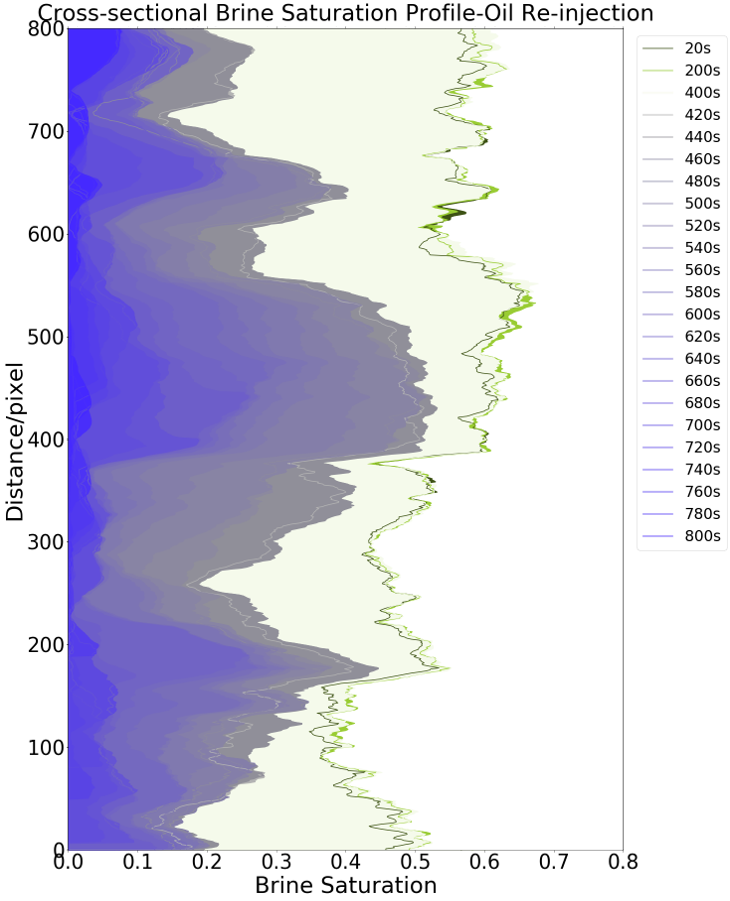
\includegraphics[width=1\textwidth]{\dir/figs/oil_satu_flip.png}
    \caption{Caption}   
    \label{oilsatu}
\end{figure}
 
\subsection{Saturation in steady-state injection}\label{subsection_sssaturation}
We observed saturation cycles in the steady-state injection. During the injection, saturation of brine increased from 1\% to 40\%, then immediately started decreasing until the brine saturation back to 1\%. Then brine saturation raised again to just below 40\% and fluctuated around 35\%-40\%. Once it surpassed 40\%, the brine saturation started to decrease back to near 5\% at the end of injection. The whole saturation change is recorded in Fig.\ref{satuall} from T=1750s ($\diamond$1) to T=2800s ($\diamond$6). The visualisations brine occupancy of $\diamond$1-6 is shown correspondingly in Fig.\ref{cycle} which shows the peak and valley saturation of the brine. 

Fig.\ref{cycle} 1 shows the CT scan taken after the oil re-injection and just before steady-state injection started. The pore was nearly fully saturated with oil except minor trapped brine droplets. At the onset of steady state injection, saturation of brine increased monotonically to 40\%. The slope of this brine saturation increase (Fig.\ref{satuall} $\diamond$1-2) is very close to that of the brine injection (Fig.\ref{satuall} T=0s-400s). In the brine injection the brine was injected at the rate of 2.5\textmu l/min, and in steady-state the oil and brine were co-injected both at 2.5\textmu l/min, which means the total flow of mass was doubled. To achieve the same increasing slope in steady-state injection, the oil flow must not interfere with the amount of brine injected, otherwise the slope of brine saturation will be less steep. 

Two phase flow experiments in bead packs and micromodels at low capillary numbers show that wetting and non-wetting fluids have separate flow pathways \citep{lenormand1983mechanisms, chatenever1952visual}, these flow pathways remain stable once established. In the context of our study, this is indirectly supported by the fact that the oil flow did not interfere with the amount of brine being injected, this is implied by the same slope of brine saturation change in brine injection and steady-state injection.

\citet{datta2014fluid} reported that at higher flow rate the non-wetting phase can break up into discrete ganglia and advect through the pore system by the wetting fluid. This was discovered in a 3D model porous medium. In natural sandstone, \citet{reynolds2017dynamic} found that in steady-state flow with high capillary number ($C_a$ close to $10^{-5}$), the non-wetting phase can constantly rearrange the connection between filled pores. These findings imply a more dynamic flow behaviour in steady-state flow than the stable pathway that is typically assumed. The non-wetting pathway can be rearranged in multiple ways. In our steady-state flow results, we do see this dynamic change of pathways. It is suggested by the fact that brine saturation did not stabilise after first reaching 40\%, but oscillate cyclic between 1\% and 40\% (Fig.\ref{satuall} $\diamond1-6$, Fig.\ref{cycle} 1-6). 

In this study, for the wetting phase that can freely flow throughout the pore system using the crevices, micropores and roughness, the pathway is difficult to identify under the current resolution. But for the non-wetting phase, the brine, we can clearly see the major change of pathway in Fig.\ref{centralchannel}. Due to the lack of access on the inlet face, minor change of pathway at the inlet face, can bring drastic change to the flow inside the target zone. The change of the pathway on the inlet face can not be ultimately tracked down to the buffer zone below the target zone, but we assume that some dynamic switching of non-wetting fluid connectivity, as \citet{reynolds2017dynamic} described, occurred below the inlet face and caused this change of pathway. The change of pathway on the inlet face caused the major switch of imbibition and drainage in the target zone. When the central channel was connected with the brine pathway under the inlet face, a pathway of brine started to establish because of the continuous supply of brine, thus led to brine saturation increase. When the connection to brine was cut, the supply of brine at the central channel was cut and the continuously flowing oil quickly snapt-off to adapt to the new capillary equilibrium, the snap-off lead to fast filling of the throat and therefore established an oil pathway which caused the brine saturation decrease.

The trigger of this switch, is believed to be correlated with the relative saturation in the target volume. Fig.\ref{satuall} shows that at $\diamond2,3,5$ when the brine saturation reached local minimum and maxima, the saturation instantly switched towards opposite trend. And the saturation trend did not change in the middle of a trend until it reached the extreme. This can be explained by the change of relative permeability which is dependent on the relative saturation. When the brine saturation was increasing, the relative permeability of oil ($k_ro$) dropped sharply, and caused the accumulation of oil pressure at the inlet face. When it reached a critical pressure for snap-off, the throat of the central channel on the inlet face was quickly filled with oil and starting to establish the wetting phase pathway, the pathway flow of oil then started to displace the brine in place($\diamond2$). The brine saturation was then decreased. And vice versa, the decreased saturation of the non-wetting phase lead to the decrease of relative permeability of water ($k_rw$). Again when the critical capillary entry pressure of brine was accumulated, brine started to invading the central channel again ($\diamond3$). At Fig.\ref{satuall} $\diamond4-5$, the brine saturation experienced fluctuation, and eventually built up the thresholding saturation that caused the corresponding critical pressure that lead to the switch.

\subsubsection{Intermittent fluid pathway}
The intermittency of fluid pathway in steady state flow is highly similar with \citet{spurin2019intermittent}'s finding. They conducted steady state core flooding experiment in a heterogeneous, water-wet carbonate rock, and observed intermittent pathway flow in intermediate-sized pores at low capillary numbers due to the competition between two fluid phases. Such intermittency leads to the interrupted transport of one fluid, and allows the establishment of the other fluid. \citet{spurin2019intermittent} also reported that higher heterogeneity encourages intermittent pathway flow, which agrees with our observation in the highly heterogeneous Indiana limestone. This study confirmed the occurrence of the intermittent fluid pathway in mixed-wet heterogeneous pore system.

The two fluids had not reached equilibrium saturation within the observation window of the steady-state injection. The relative saturation of two fluids formed a typical bi-stable system where the critical relative saturation of one fluid act as the activation of the critical condition of another fluid to enter the system. The relative permeability provides positive feedback to the capillary entry pressure and the single channel on the inlet face prevented increase without bound. In such bi-stable system, relative saturation of two fluids will not reach static equilibrium but switch between imbibition and drainage if the injection maintains stable.

\begin{figure}
    \centering
    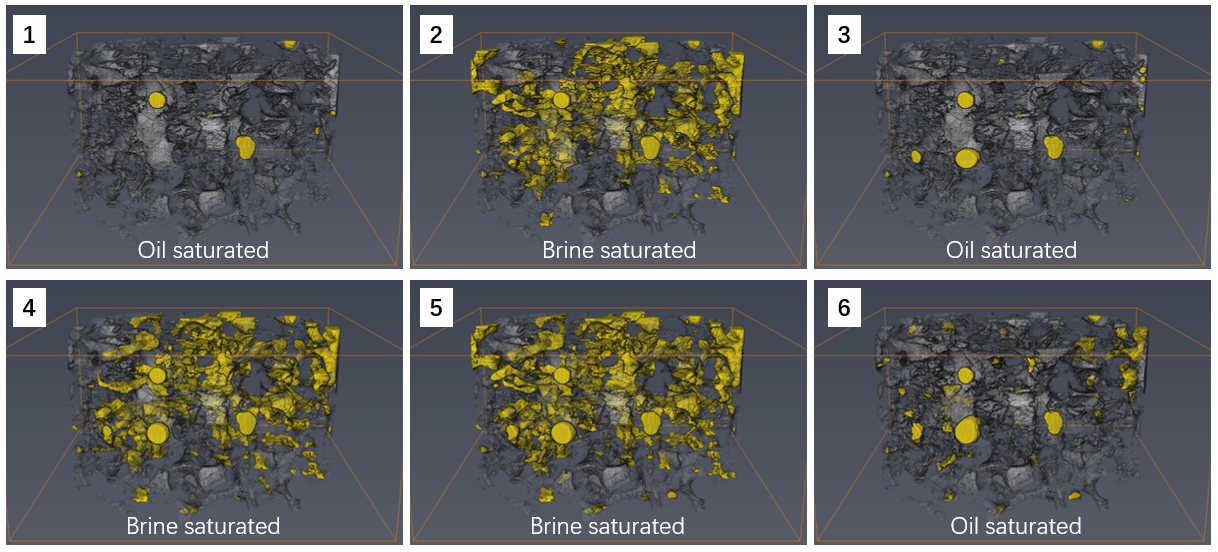
\includegraphics[width=1\textwidth]{\dir/figs/cycle}
    \caption{Caption}
    \label{cycle}
\end{figure}

\section{Throat characterisation and fluid path}
Pore throat is the narrower conduit between two wider pore bodies, in some study such as pore network modelling, it is convenient to describe and characterise a throat as a surface, which is the narrowest restriction that defines the boundary between two pore regions (e.g. \citet{singh2016imaging,wildenschild2013x}). Treating a pore throat as a surface works well in homogeneous porous media such as bead packs and sand stones, because in these pore system, pore throats are typically the restrictions where spherical grains compactify. However in a heterogeneous pore system, throats can be tortuous and irregular, thus it requires a body rather than a surface to represent.

\subsection{Pore body-throat partition}
With the method described in Chapter 3, it is able to identify pore throats as a thin body that connects two wider pores. Fig.\ref{throat2d} shows the throats identified in 2D image slice (left), and 3D rendering of throats that connecting the wider pores (right). 

\begin{figure}
    \centering
    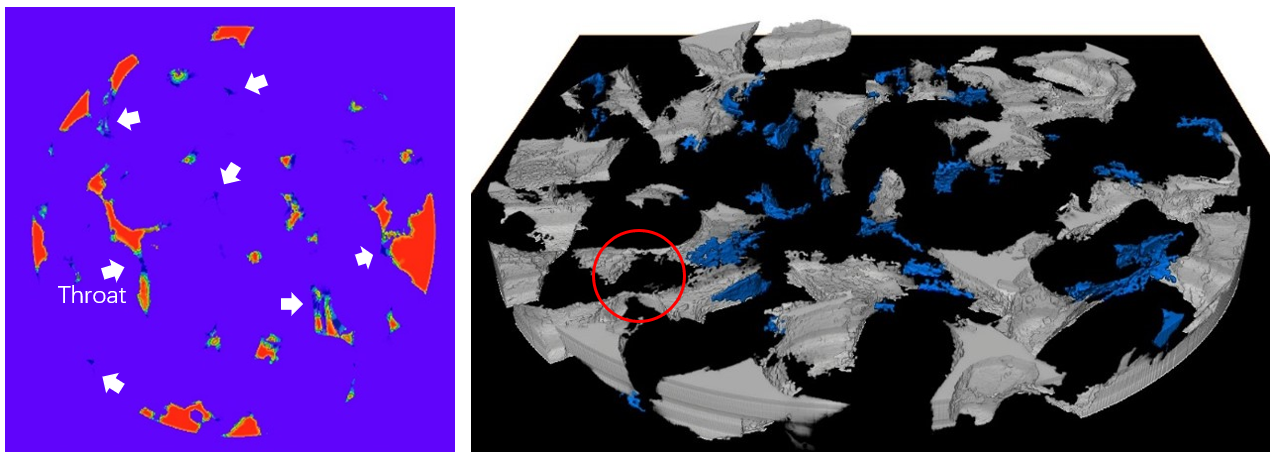
\includegraphics[width=1\textwidth]{\dir/figs/throat2d}
    \caption{Caption}
    \label{throat2d}
\end{figure}

In order to define throat, first we need to define pore body. Pore body is defined by performing euclidean distance transform in 3D pore space. The outcome is a distance map that mapping the value of euclidean distance to the closest boundary from each voxel. Because pores are locally wider than throats, so pores generally have higher distance value than throats. Bear in mind that The pore system is heterogeneous and multi-scale, some throats can be even larger than some pore bodies compared globally. So classical adaptive thresholding by Niblack and Sauvola \citep{niblack1985introduction, sauvola2000adaptive} is used to find the local minima and maxima that representing the centre of throats, and the centre of pore bodies, at local regions. In conclusion, the centre of pore bodies are defined by the local maxima of 3D euclidean distance, and the centre of throats are defined by the local minima of 3D euclidean distance.

Having found the centres of pore bodies and throats, the following step is to define the pore bodies and throats at each centre. I used the seeded random walker algorithm (\citet{grady2005multilabel}, described in Chapter 3) to fill the regions of throats and pore bodies. Treating as irregular bodies, the transition from pore body to throats is always gradational. Therefore, rather than using a hard segmentation that unequivocally defines throats and bodies, I used probability map produced by random walker to represent the transition. For example in Fig.\ref{throat2d}, pore space that labelled red has high probability of being a pore body, and those labelled blue is of high probability of being a pore throat. Between these high probability regions, intermediate probability is labelled with gradation colours to represent the transition from pore body to throat, where the definition of belonging of throat or pore body is ambiguous. I believe this is the suitable and proper characterisation of throats and bodies in such heterogeneous pore system.

The characterisation has shortage. Due to the sensitivity of adaptive thresholding, chance existed that throats can be missed. Such as some throats shown on Fig.\ref{throat2d} right were not correctly picked out (red circle).

\paragraph{Throat size characterisation}
Throat when characterised as a 3D surface, the size of it can be characterised by few parameters such as the radius of a circle or the eccentricity of an ellipse and the curvature if the surface is curved. Throat when defined as an irregular body, becomes more difficult to be characterised. 

In the context of this study, for simplicity we generally consider throats as a circular, elongated conduit with varied radius alone the long axis, more complex features such as tortuousity or eccentricity are not taking into account. The radii are measured by max inscribed spheres (MIS) method. The algorithm was operated in 3D to calculate the maximum radius of the inscribed sphere at each voxel (a 2D slice of MIS is shown in Fig.\ref{maxball}). The size of one throat is characterised statistically by the mean, mode and major radius of it. The minimum radius is not taken into account because it measures the smallest crevices and surface roughness instead of the apparent narrowest radius of the throat. For measuring the apparent narrowest restriction radius, \citet{singh2016imaging,wildenschild2013x}'s method can be adopted.

\begin{figure}
    \centering
    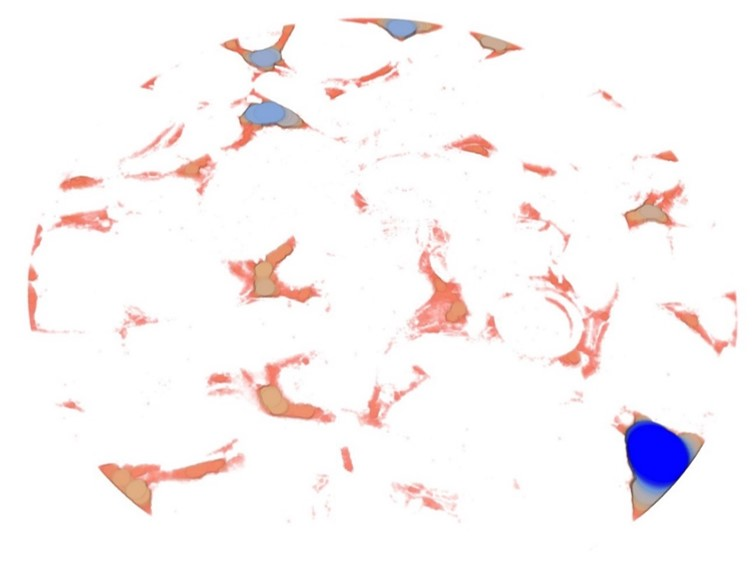
\includegraphics[width=1\textwidth]{\dir/figs/maxball}
    \caption{Caption}
    \label{maxball}
\end{figure}

\subsection{Fluids in the throat}
\begin{figure}
    \centering
    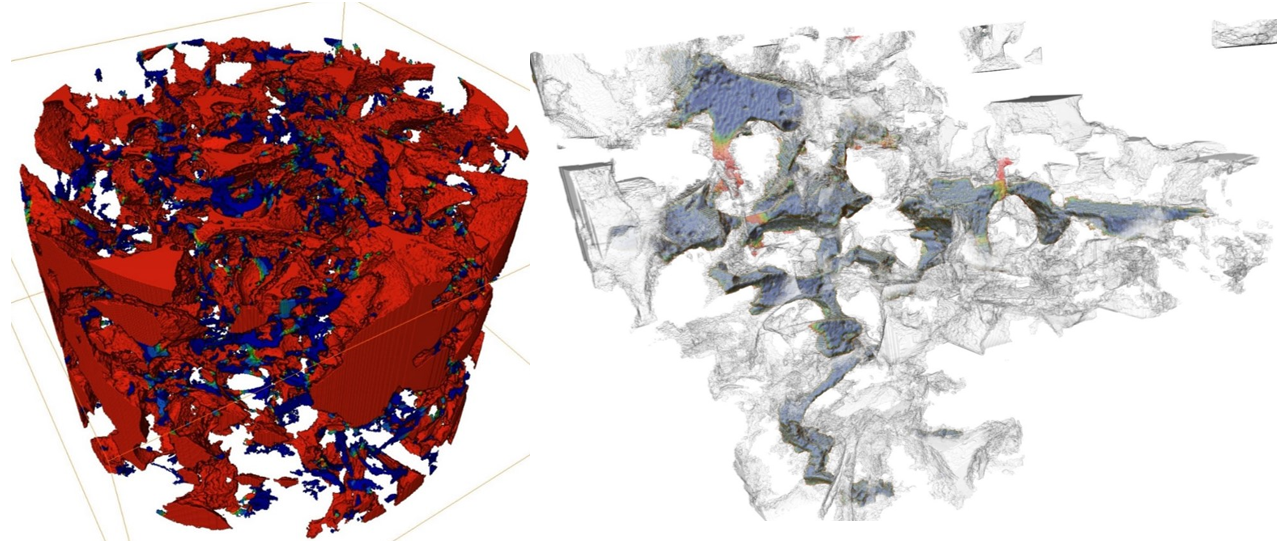
\includegraphics[width=1\textwidth]{\dir/figs/throat3d}
    \caption{Caption}
    \label{throat3d}
\end{figure}
In Fig.\ref{throat3d} left, I have visualised the throats (blue) that connecting the pore bodies (red) throughout the target volume. It shows a highly connected network with very irregular geometry. 

To investigate fluid occupancy in the throats, I superimpose brine clusters of the early brine injection with throats to produce Fig.\ref{throat3d} right. Blue labels the brine cluster and warmer colours label the pore throats. The semi-transparent grey shows the boundary of the pore space. It visualised that at the early stage of brine injection, brine generally preferred to fill larger pores.

To further analyse the potential path of fluid flow, I investigated potential throats that adjacent to the brine cluster (Fig.\ref{passedthroats} left). The potential throats that accessible for the brine are labelled blue, the existed brine cluster is labelled grey. And by comparing with the future scans, we quantified the population of throats that were passed by the brine, and those were un-passed. The quantification is shown in Fig.\ref{passedthroats} right. The figure shows that the distribution of passed throats size and un-passed throats size are overlapping, but bins of passed throat size generally shifts to the right side of the un-passed throats, meaning that for different range of throat sizes, brine generally passed through those relatively larger throats. This shows consistency with the observation of the brine being the non-wetting fluid.

\begin{figure}
    \centering
    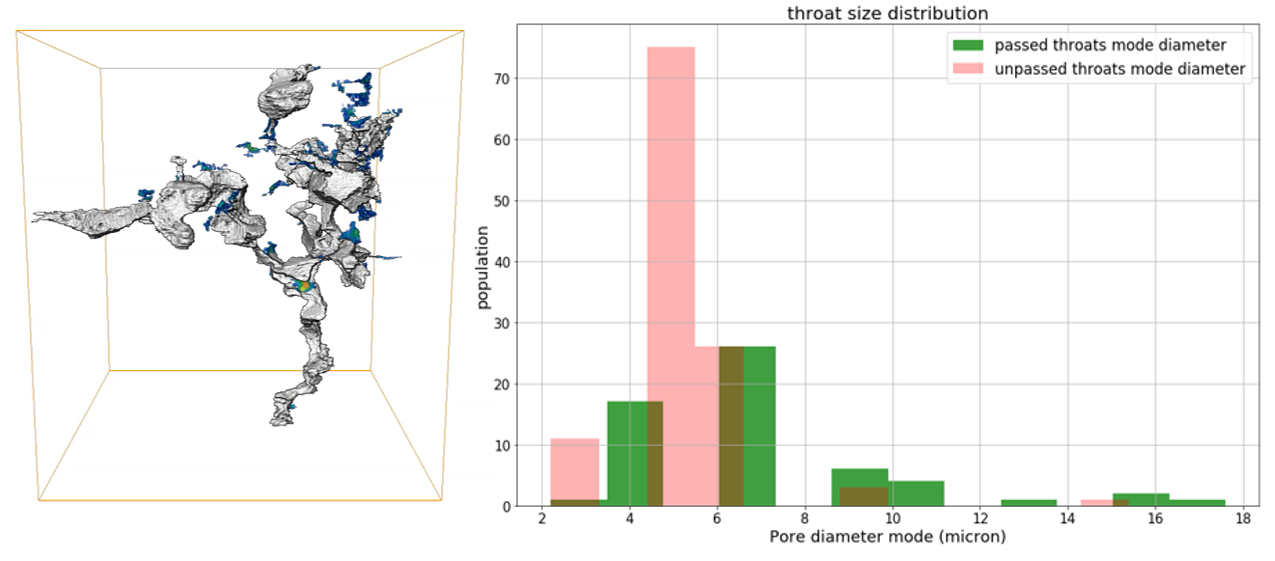
\includegraphics[width=1\textwidth]{\dir/figs/passedthroats}
    \caption{Caption}
    \label{passedthroats}
\end{figure}

This pore body-throat partitioning technique has much more potential usage than the above demonstration. With this partitioning method, more detailed geometry of pore body and throats can be characterised separately. In such highly heterogeneous and multi-scale pore system, geometry measurement such as aspect ratio, tortuousity and max inscribed sphere radius, can be very different for pore body and throats. So separating the measurements can be crucial for deeper understanding of carbonate pore network.

\section{Fluid connectivity analysis}
\subsection{Connectivity of brine and oil during drainage}
The fluid connectivity of brine and oil are quantified by calculating the Euler number at each injection experiment. Theoretically, during a drainage process, brine as the non-wetting phase is connected by flow pathways and disconnected by Roof snap-off events. And during imbibition, brine was disconnected by snap-off events. I measure the connectivity of brine to study how the non-wetting fluid is connected and disconnected during different stages of injections. The Euler number is conventionally normalised with volume as a measurement of connectivity per unit volume.

Fig.\ref{brine_connectivity} shows brine connectivity during brine injection. As brine saturation increasing, the normalised Euler number decreased from near-zero to -7000. Positive Euler number implies discrete droplets and low connectivity and negative Euler number implies connected fluid clusters. The statistics shows that as brine injected into oil saturated core, the fluid body was establishing more and more inter-connected pathways through the larger pore space. There is a linear relationship between the relative brine saturation and its connectivity.

\begin{figure}
    \centering
    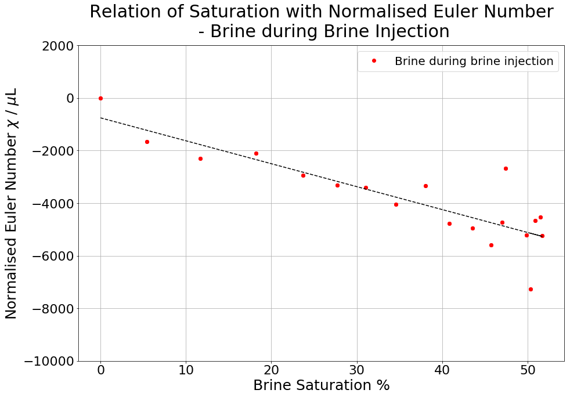
\includegraphics[width=1\textwidth]{\dir/figs/brine_connectivity.png}
    \caption{Caption}   
    \label{brine_connectivity}
\end{figure}

The connectivity of oil during brine injection was measured as brine's counterpart. The Euler number measurement shows in Fig.\ref{oil_connectivity}. The relative saturation of oil decreased from 100\% to less than 50\%. During the de-saturation of oil, the Euler number measured on oil decreased from -10000 to -15000, meaning increasingly connected oil body. The result suggests that the wetting phase connectivity can increase while its saturation decreased, during non-wetting phase invasion. 

\begin{figure}
    \centering
    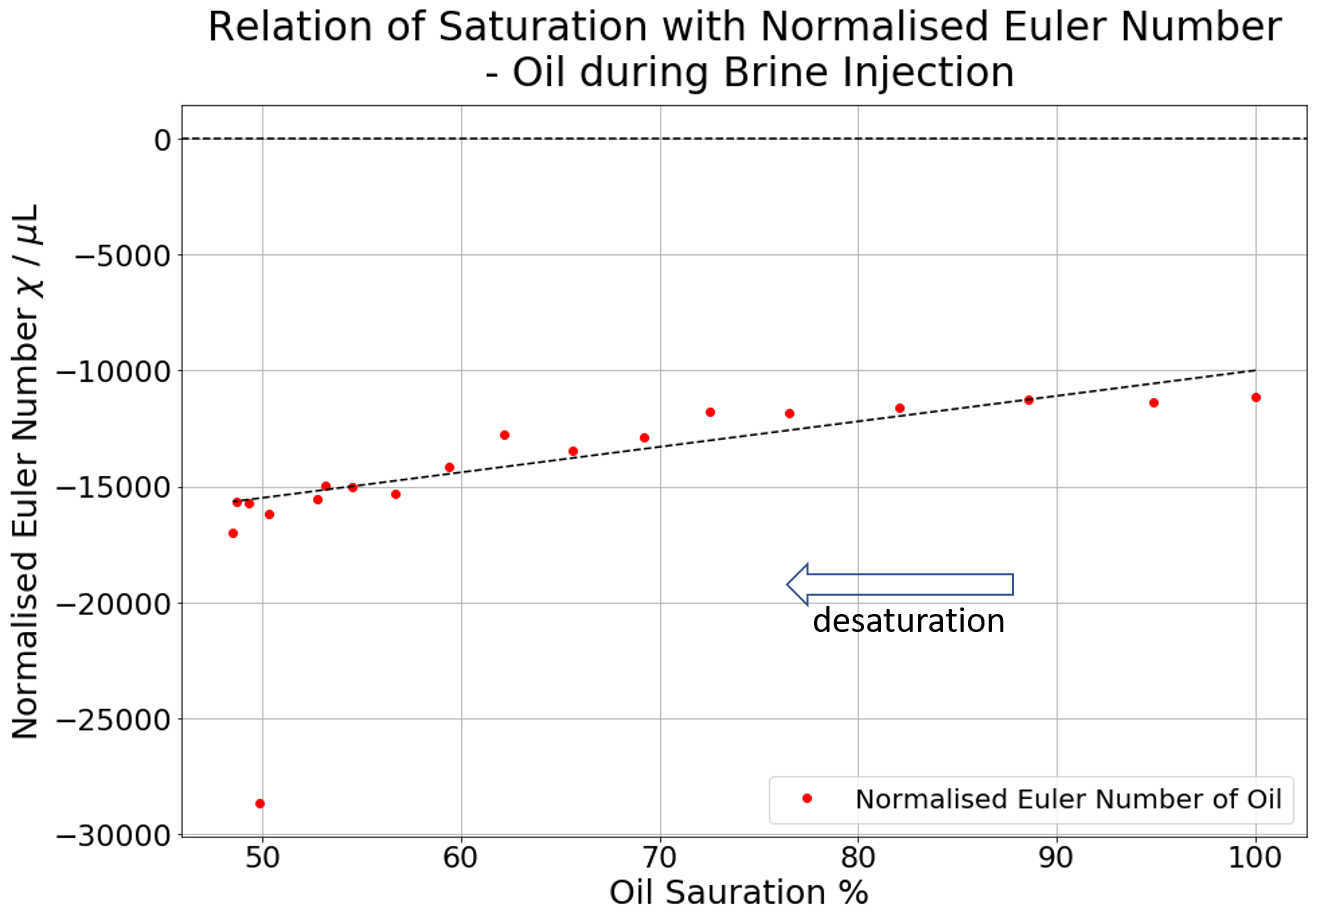
\includegraphics[width=1\textwidth]{\dir/figs/oil_connectivity.png}
    \caption{Caption}   
    \label{oil_connectivity}
\end{figure}

The connectivity is increased by establishing more inter-connected wetting layers, example shows in Fig.\ref{wettinglayers}. In Fig.\ref{wettinglayers} upper two images shows the 3D rendering of oil, at T=40s when the brine started entering the pore system, and at T=400s when the residual oil reached irreducible saturation. At T=40s, the oil body was connected throughout the pore space. After the brine injection, the oil stay connected throughout the pore space. The original connection was replaced by much finer structures with more population. Such finer connective structures are the wetting layers, example shown in Fig.\ref{wettinglayers} lower two images. The images are one slice of raw CT image of two macro pores after brine injection and its segmentation. The brine occupied the centre of the pores, but due to the non-wetting nature of the brine in this pore system, the brine was unable to fully occupy the fine throat connecting the two pores and the crevices at the corners (pointed with red arrow). Oil as the wetting fluid stay resided in the crevices as wetting layers to maintain the oil connectivity. As a result, the original one unified connection of oil was split into several more connections. This explains how oil connectivity increased while its saturation decreased.   

\begin{figure}
    \centering
    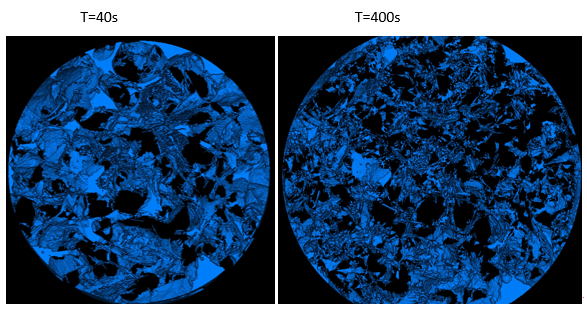
\includegraphics[width=1\textwidth]{\dir/figs/connectivity3d}
    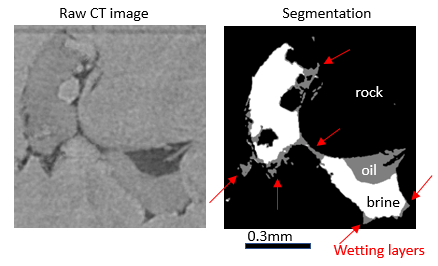
\includegraphics[width=1\textwidth]{\dir/figs/wettinglayers}
    \caption{Caption}   
    \label{wettinglayers}
\end{figure}

Oil as the main wetting phase, should largely connected throughout the pore space with wetting films and wetting layers, and inter-connected micro-pores. The spatial resolution of imaging in this study is insufficient to identify the wetting films and micro pores, only wetting layers are identical in this study. The genuine connectivity of oil should be higher than measured because of this limitation. Despite of the limitation, this study has stressed the role of wetting layers in connecting the wetting phase.

\subsection{Brine connectivity during imbibition}

When the brine injection ended, the core was partially saturated with oil and brine. At this time we started oil re-injection. Oil, as the main non-wetting fluid, was re-injected into the core to displace the brine in place, and the brine saturation started to decrease. The connectivity of brine during the displacement was measured by calculating its Euler number. The result is shown in Fig.\ref{brine_connectivity2}. Again due to the time gap of imaging, the beginning of oil re-injection was not captured which caused the inconsistency of end point and start point of the measurement. 

\begin{figure}
    \centering
    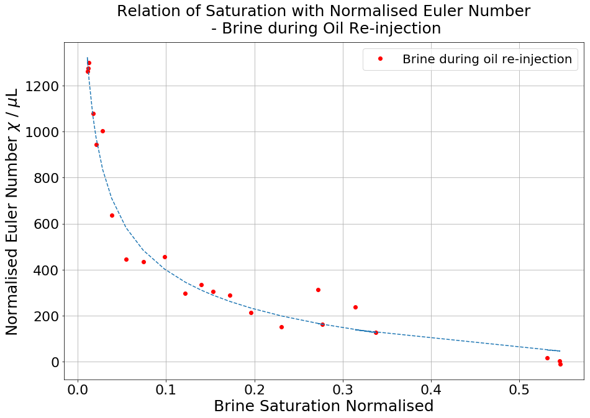
\includegraphics[width=1\textwidth]{\dir/figs/brine_connectivity2.png}
    \caption{Caption}   
    \label{brine_connectivity2}
\end{figure}

From the first CT scan of oil re-injection on, brine saturation decreased from above 0.5 to near zero. The Euler number of brine body raised from near zero to 12000. This means that, the beginning during which Euler number raised from -5000 to near zero was uncaptured by CT imaging. During the rest part of oil re-injection, brine lost its connectivity due to snap-off events and became increasingly disconnected. The increase of brine's Euler number has a power-law relation with brine's relative saturation.

\subsection{Brine's connectivity during steady state injection}
Fig.\ref{ss_connectivity} summarised the saturation of brine and its Euler number during steady state injection. The saturation of brine (blue dots) shows cyclic increasing and decreasing between 0 to 40\% due to the bi-stable switching of the central fluid channel.

The Euler number (red dots) shows connectivity of the brine during the steady state injection. The moving average of the Euler number (black dotted curve) shows mirrored response of brine's connectivity to its relative saturation. The increase of saturation leads to dropping Euler number, and the decrease of saturation leads to rising Euler number. The Euler number oscillates above and below the zero level shows that the connectivity of brine switching between discrete droplets and connected pathway. When the brine saturation increased, its bulk connectivity was increased by establishing inter-connected loops of flow pathways surrounding the oolite grains. Locally there may be lost of connectivity due to Roof snap-off events. When the wetting oil displacing brine became dominate, the brine saturation started decreasing, and its connectivity was cut by snap-off events. This reveals strong relation between the non-wetting saturation and its connectivity.

\begin{figure}
    \centering
    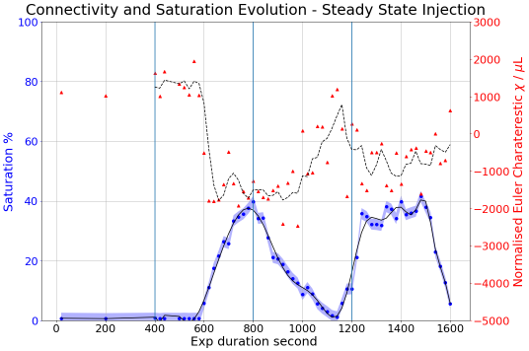
\includegraphics[width=1\textwidth]{\dir/figs/ss_connectivity.png}
    \caption{Caption}   
    \label{ss_connectivity}
\end{figure}

Brine Euler number measurements during all injection stages was plotted in Fig.\ref{brine_connectivity3}. It summarises the range of non-wetting fluid connectivity during different events. 

For the brine injection stage, it is mainly a drainage process, the Euler number measurements (red dots) span across -2000 to -7000 for relative saturation between ~5\% to ~50\%. The brine is highly connected during drainage. For the oil re-injection stage, it is mainly an imbibition process, the Euler number measurements (blue dots) are mainly positive numbers between 0 to 2000, which implies disconnected brine clusters and discrete droplets during imbibition process. For steady state injection, during which both imbibition and drainage took place, the Euler number measurements (green dots) clustered in the range in-between the former two. The Euler number measurements span across 2000 to -2000, meaning that the connectivity of brine varies from intermediately connected to discrete and unconnected.

\begin{figure}
    \centering
    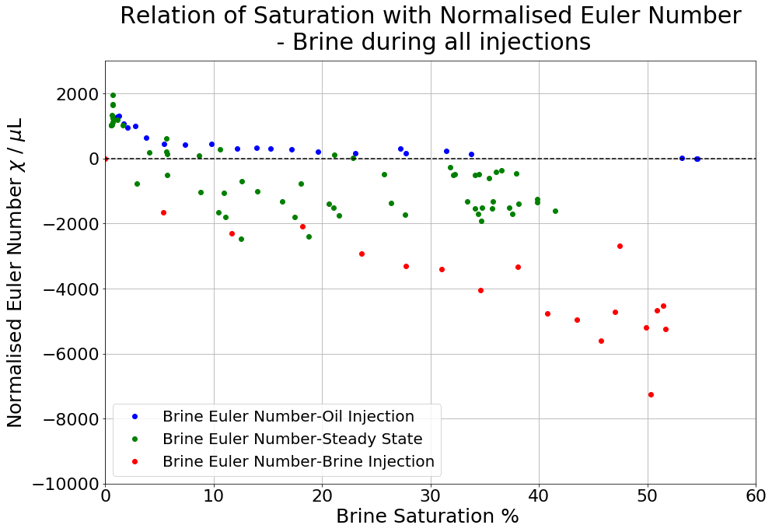
\includegraphics[width=1\textwidth]{\dir/figs/brine_connectivity3.png}
    \caption{Caption}   
    \label{brine_connectivity3}
\end{figure}

Similar study was reported by \citet{khanamiri2018fluid}. The study was conducted in a water-wet Berea sandstone. 

Their results showed that, in general, the non-wetting fluid Euler number is proportional to the wetting fluid saturation. Indicating the higher wetting fluid saturation is resulted in lower non-wetting fluid connectivity. In their study, during imbibition when the wetting fluid saturation increased, the Euler number of the non-wetting fluid increased too, indicating more disconnected topology. Their study also shows that during drainage when the wetting fluid saturation decreased, the Euler number of the non-wetting fluid decreased too. Which is consistent with our study.

For wetting fluid connectivity during drainage, their results showed non-wetting connectivity increased while the wetting phase saturation increased, which is opposite to our result in this thesis. This shows the essential difference of non-wetting fluid connectivity in Berea sandstone with more heterogeneous Indiana limestone.
 
\section{Modelling of a pore scale event: Roof snap-off}\label{modelling}
A Roof snap-off event during brine injection (drainage) was identified. The event took around 40s, Fig.\ref{roofsnapoff} shows the specific pore of the Roof snap-off event. At injection time=60s, brine (blue) started migrating to the larger pore on its left, and the next scan captured the Roof snap-off event where the non-wetting brine was snapped-off by the wetting film. The third scan captured the end of the event that the non-wetting brine eventually filled the throat and continually feeding through it.

\begin{figure}
    \centering
    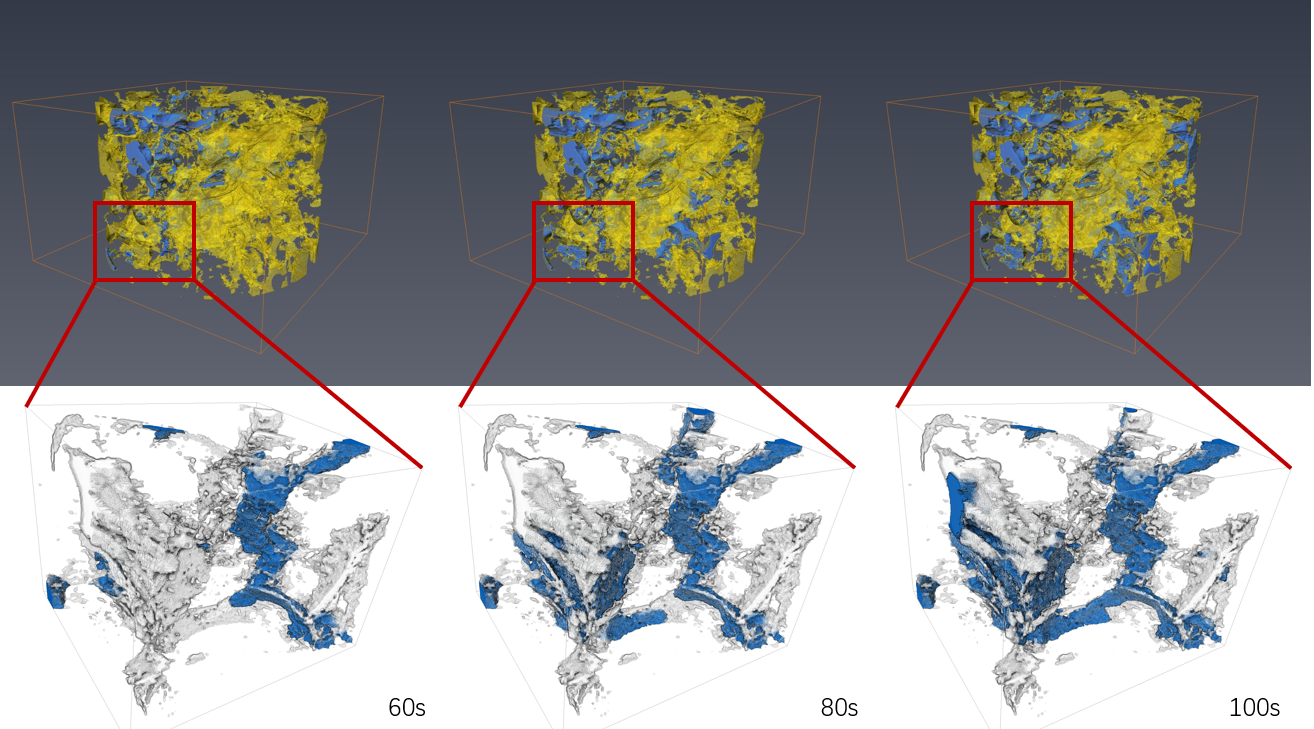
\includegraphics[width=1\textwidth]{\dir/figs/roofsnapoff.png}
    \caption{Caption}   
    \label{roofsnapoff}
\end{figure}

This Roof snap-off process was numerically modelled and repeated by modelling method by Dr.Julien Maes from the Heriot-watt University. The work was direct numerical simulation (DNS) by Volume-of-Fluid (VOF,\citep{hirt1981volume}) method. 

\subsection{Roof snap-off criteria}
\citet{roof1970snap} first time described the quasi-static criterion for Roof snap-off to occur in a circular pore:

\begin{equation}
    \frac{1}{R_{p}} < \frac{1}{R_{t}} + \frac{1}{R_{zt}}
\end{equation}

where $R_p$ is the effective pore radius, $R_t$ is the effective throat radius, $R_{zt}$ is the curvature radius that transverse the throat. In the context of this study $R_{zt}$ is much larger than $R_t$ thus $\frac{1}{R_{zt}}$ is insignificant. This criterion was used as a necessary condition to find the pore system that suitable for Roof snap-off to occur.

A pore network was extracted from the CT image to numerically represent the pore structure using the network extraction code Pnextract (https://github.com/aliraeini/pnextract,\citet{dong2009pore,bultreys2018validation,raeini2017generalized}). Fig.\ref{network} shows the visualisation of the pore network, two snap-off-possible locations were labelled on the figure, one with $R_p=10.7, R_t=5.4$, another with $R_p=13.3,R_t=6$. Only the second location with $R_p=13.3,R_t=6$ satisfies the necessary condition of a Roof snap-off event. However the condition is not always sufficient, so DNS is used to identify entry pressures and critical contact angles of the occurrence of a Roof snap-off event.

\begin{figure}
    \centering
    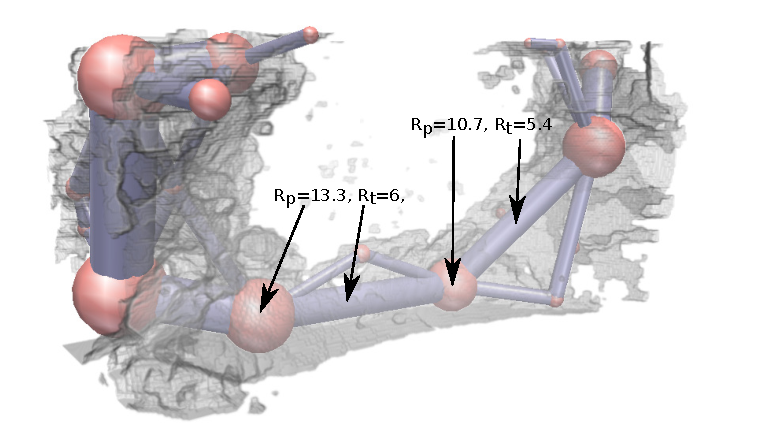
\includegraphics[width=1\textwidth]{\dir/figs/network-eps-converted-to.pdf}
    \caption{Caption}   
    \label{network}
\end{figure}

\subsection{Direct Numerical Simulation}
In direct numerical simulation, we must solve the Navier-Stokes equations in order to know how fluids flow in the pore system. The Navier-Stokes equation (N-S equation) is essentially the expression of Newton's second law of motion ($F=ma$) applied to a continuous fluid \citep{blunt2017multiphase}. The N-S equation has many formalism, its components are depending on the context of the fluid physical properties (e.g. Newtonian fluid or non-Newtonian fluids, compressible or incompressible etc.). Here in the context of this simulation Maes used a single-field formalism of N-S equation:

\begin{equation}\label{NSEVOF}
\begin{aligned}
&\nabla\cdot \mathbf{u}  = 0, \\
&\rho\left(\frac{\partial \mathbf{u}}{\partial t}+ \mathbf{u}\cdot\nabla \mathbf{u}\right)=-\nabla p + \nabla\cdot\left(\mu\left(\nabla \mathbf{u} + \nabla \mathbf{u}^T\right)\right)+\mathbf{f}_{st},
\end{aligned}
\end{equation}

The N-S equation set has two equations that the first equation $\nabla\cdot \mathbf{u}  = 0$ invokes the conservation of mass and the second equation invokes the conservation of momentum, where $\mathbf{u}$ is the single-field velocity, $p$ is the fluid pressure, $\rho$ is fluid density and $\mu$ for viscosity.

In the second equation $\rho\left(\frac{\partial \mathbf{u}}{\partial t}+ \mathbf{u}\cdot\nabla \mathbf{u}\right)$ represent the inertia of the fluid, $\frac{\partial \mathbf{u}}{\partial t}$ is the unsteady acceleration and $\mathbf{u}\cdot\nabla \mathbf{u}$ is the convective acceleration. On the right side of the equation $\nabla p $ is the pressure gradient of fluid, $\nabla\cdot\left(\mu\left(\nabla \mathbf{u} + \nabla \mathbf{u}^T\right)\right)$ represent the viscosity. $\mathbf{f}_{st}$ is the capillary forces.

The capillary forces $\mathbf{f}_{st}$ is modelled using the Continuum Surface Force (CSF) formulation introduced by \cite{brackbill1992continuum}:

\begin{equation}
 \mathbf{f}_{st}=\gamma\kappa\nabla\alpha,
\end{equation}
where $\gamma$ is the interfacial tension between the two fluids, and
$\kappa$ is the mean interface curvature, which can be computed as
\begin{equation}
 \kappa = \nabla\cdot \mathbf{n}_{12},
\end{equation}
$\mathbf{n}_{12}$ is the interface normal vector defined as:
\begin{equation}
\mathbf{n}_{12} = \frac{\nabla\alpha}{||\nabla\alpha||}.
\end{equation}

The dimensionless capillary number $C_a$ is defined as follows:

\begin{equation}
 C_a=\frac{\mu u}{\gamma},
\end{equation}

$C_a$ indicates the ratio of viscous to capillary effects at pore scale. However, $C_a$ needs to be multiplied by some geometry and saturation-dependent quantities to find the genuine ratio of viscous to capillary effects \citep{blunt2017multiphase}.

All numerical simulations were performed on GeoChemFoam, the OpenFoam-based \citep{weller1998tensorial} pore-scale two-phase flow simulator developed at Heriot-Watt University \citep{Geochemfoam}.

\subsection{Simulation parameters}
\subsubsection{Grid convergence resolution}
A computational domain of size 0.22mm$\times$0.24mm$\times$0.42mm was constructed at grid resolution of 3.6$\mu$m (Fig.\ref{domain}). This domain was used to perform the Roof snap-off simulation. We assume that the domain was initially saturated with dodecane prior to the simulation injection. 

\begin{figure}
    \centering
    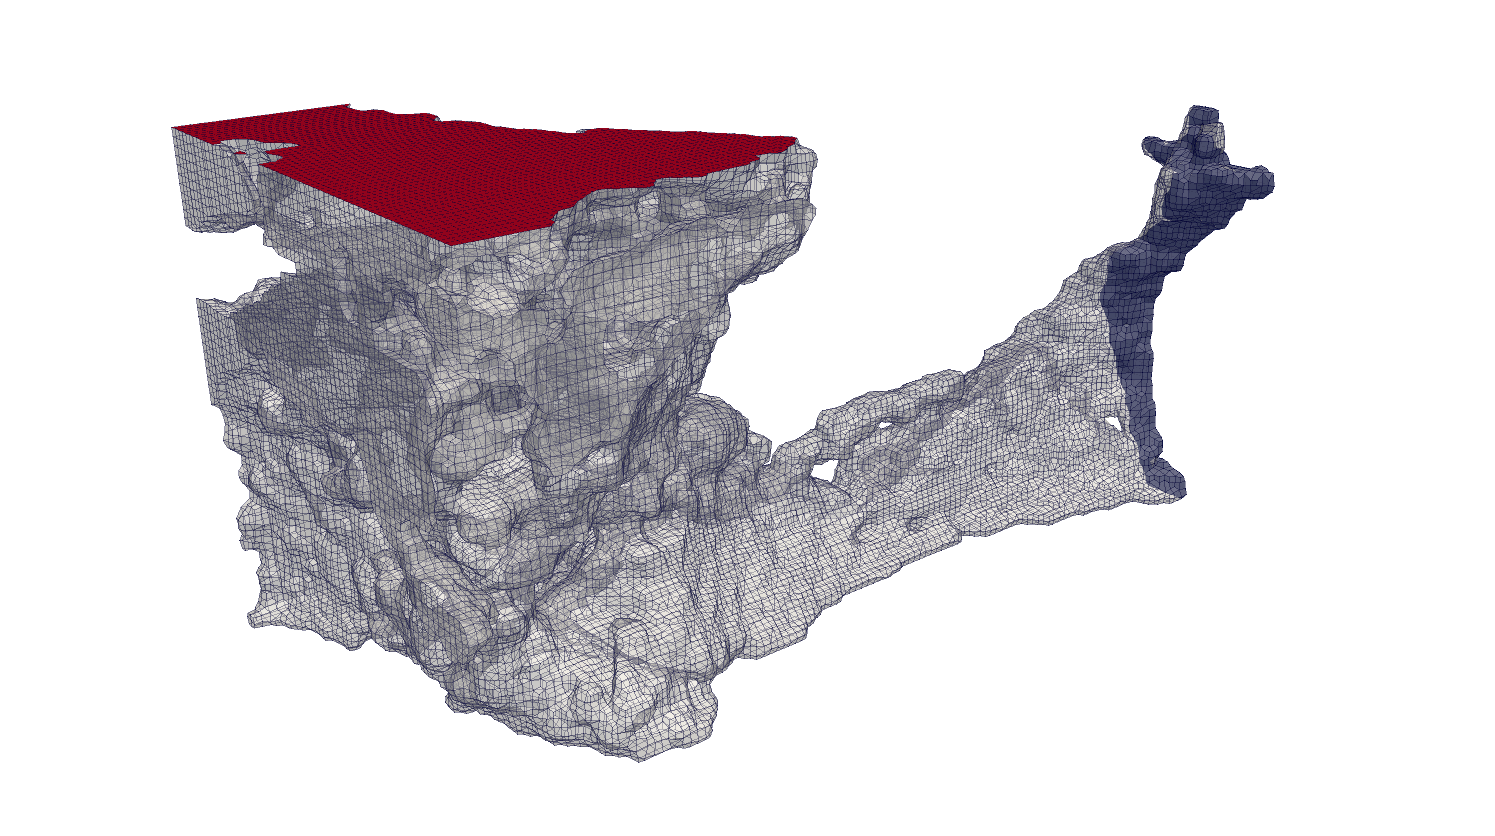
\includegraphics[width=1\textwidth]{\dir/figs/domain.png}
    \caption{Caption}   
    \label{domain}
\end{figure}

Coarser grid resolution of 5.4 $\mu$m and finer resolution of 2.4$\mu$m were also tested. Fig.\ref{pressuredropconv} shows the pressure drop between inlet (Fig.\ref{domain} blue surface) and outlet (Fig.\ref{domain} red surface). The simulation reached convergence for both intermediate and finer resolution. The intermediate resolution was used as the final grid resolution for smaller computational cost.

\begin{figure}
    \centering
    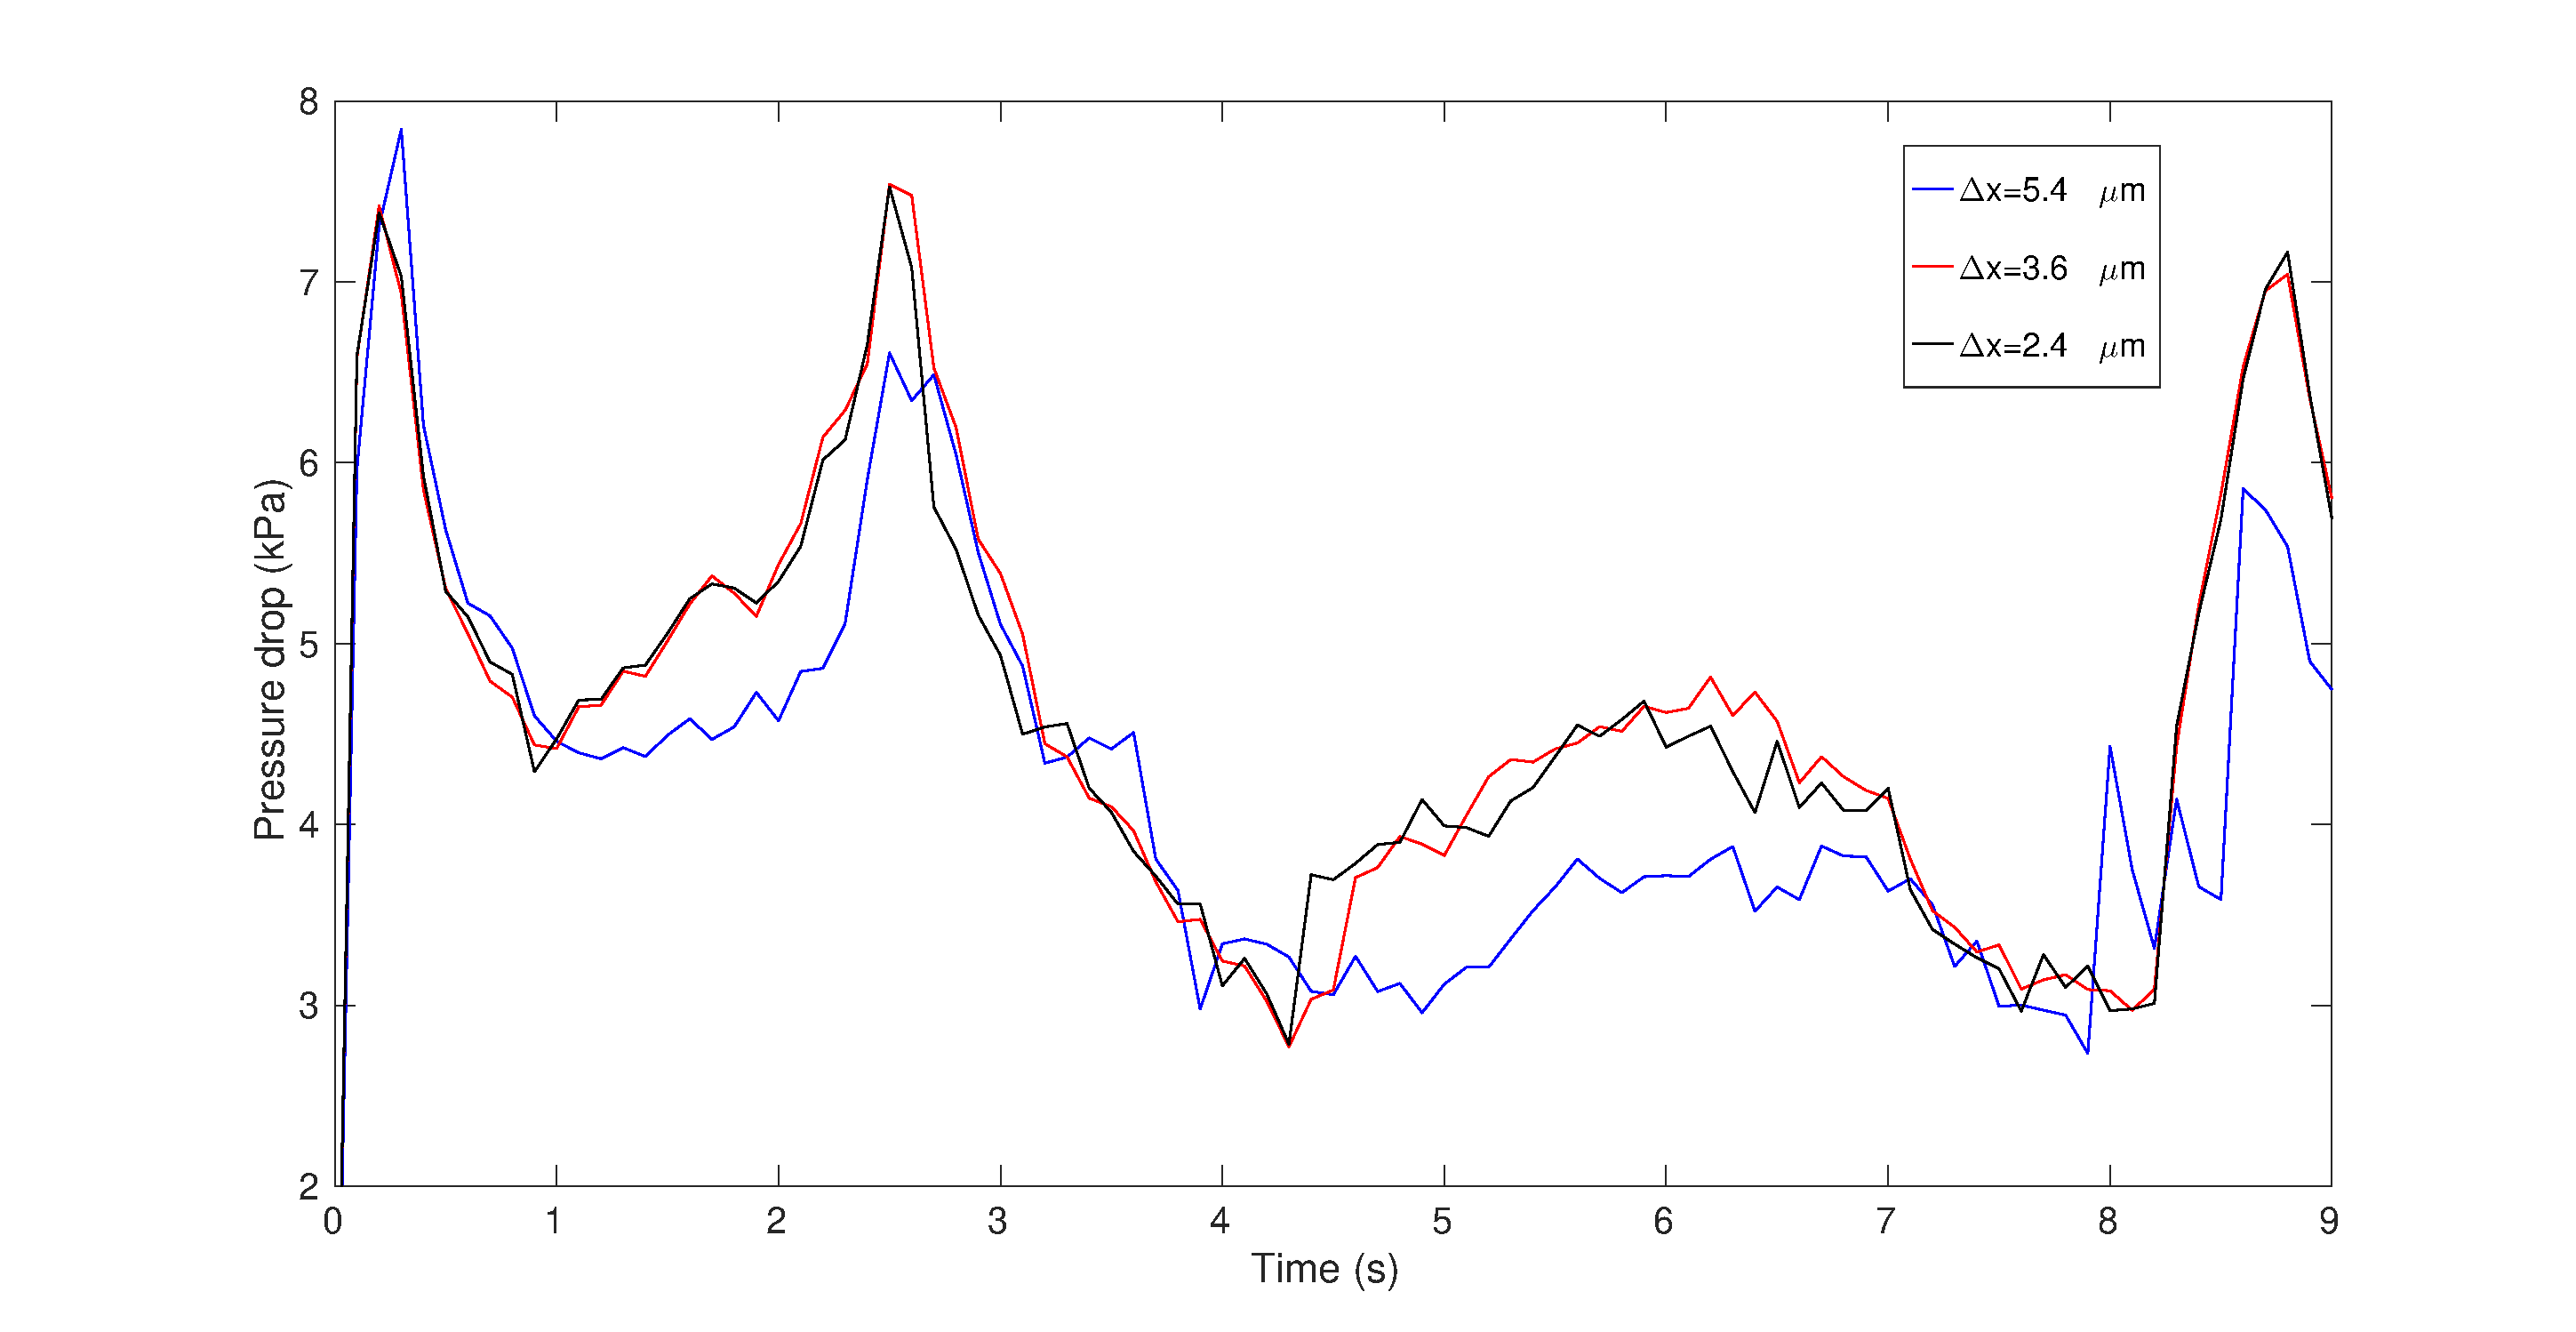
\includegraphics[width=1\textwidth]{\dir/figs/PressureDropConv-eps-converted-to.pdf}
    \caption{Caption}   
    \label{pressuredropconv}
\end{figure}

\subsubsection{Contact angle}
The effect of varied contact angles on Roof snap-off was investigated. Three contact angles: 35$^\circ$, 40$^\circ$ and 45$^\circ$ were tested. The simulation pressure drop curves for these three contact angles are plotted in Fig.\ref{pressuredrop}.

\begin{figure}
    \centering
    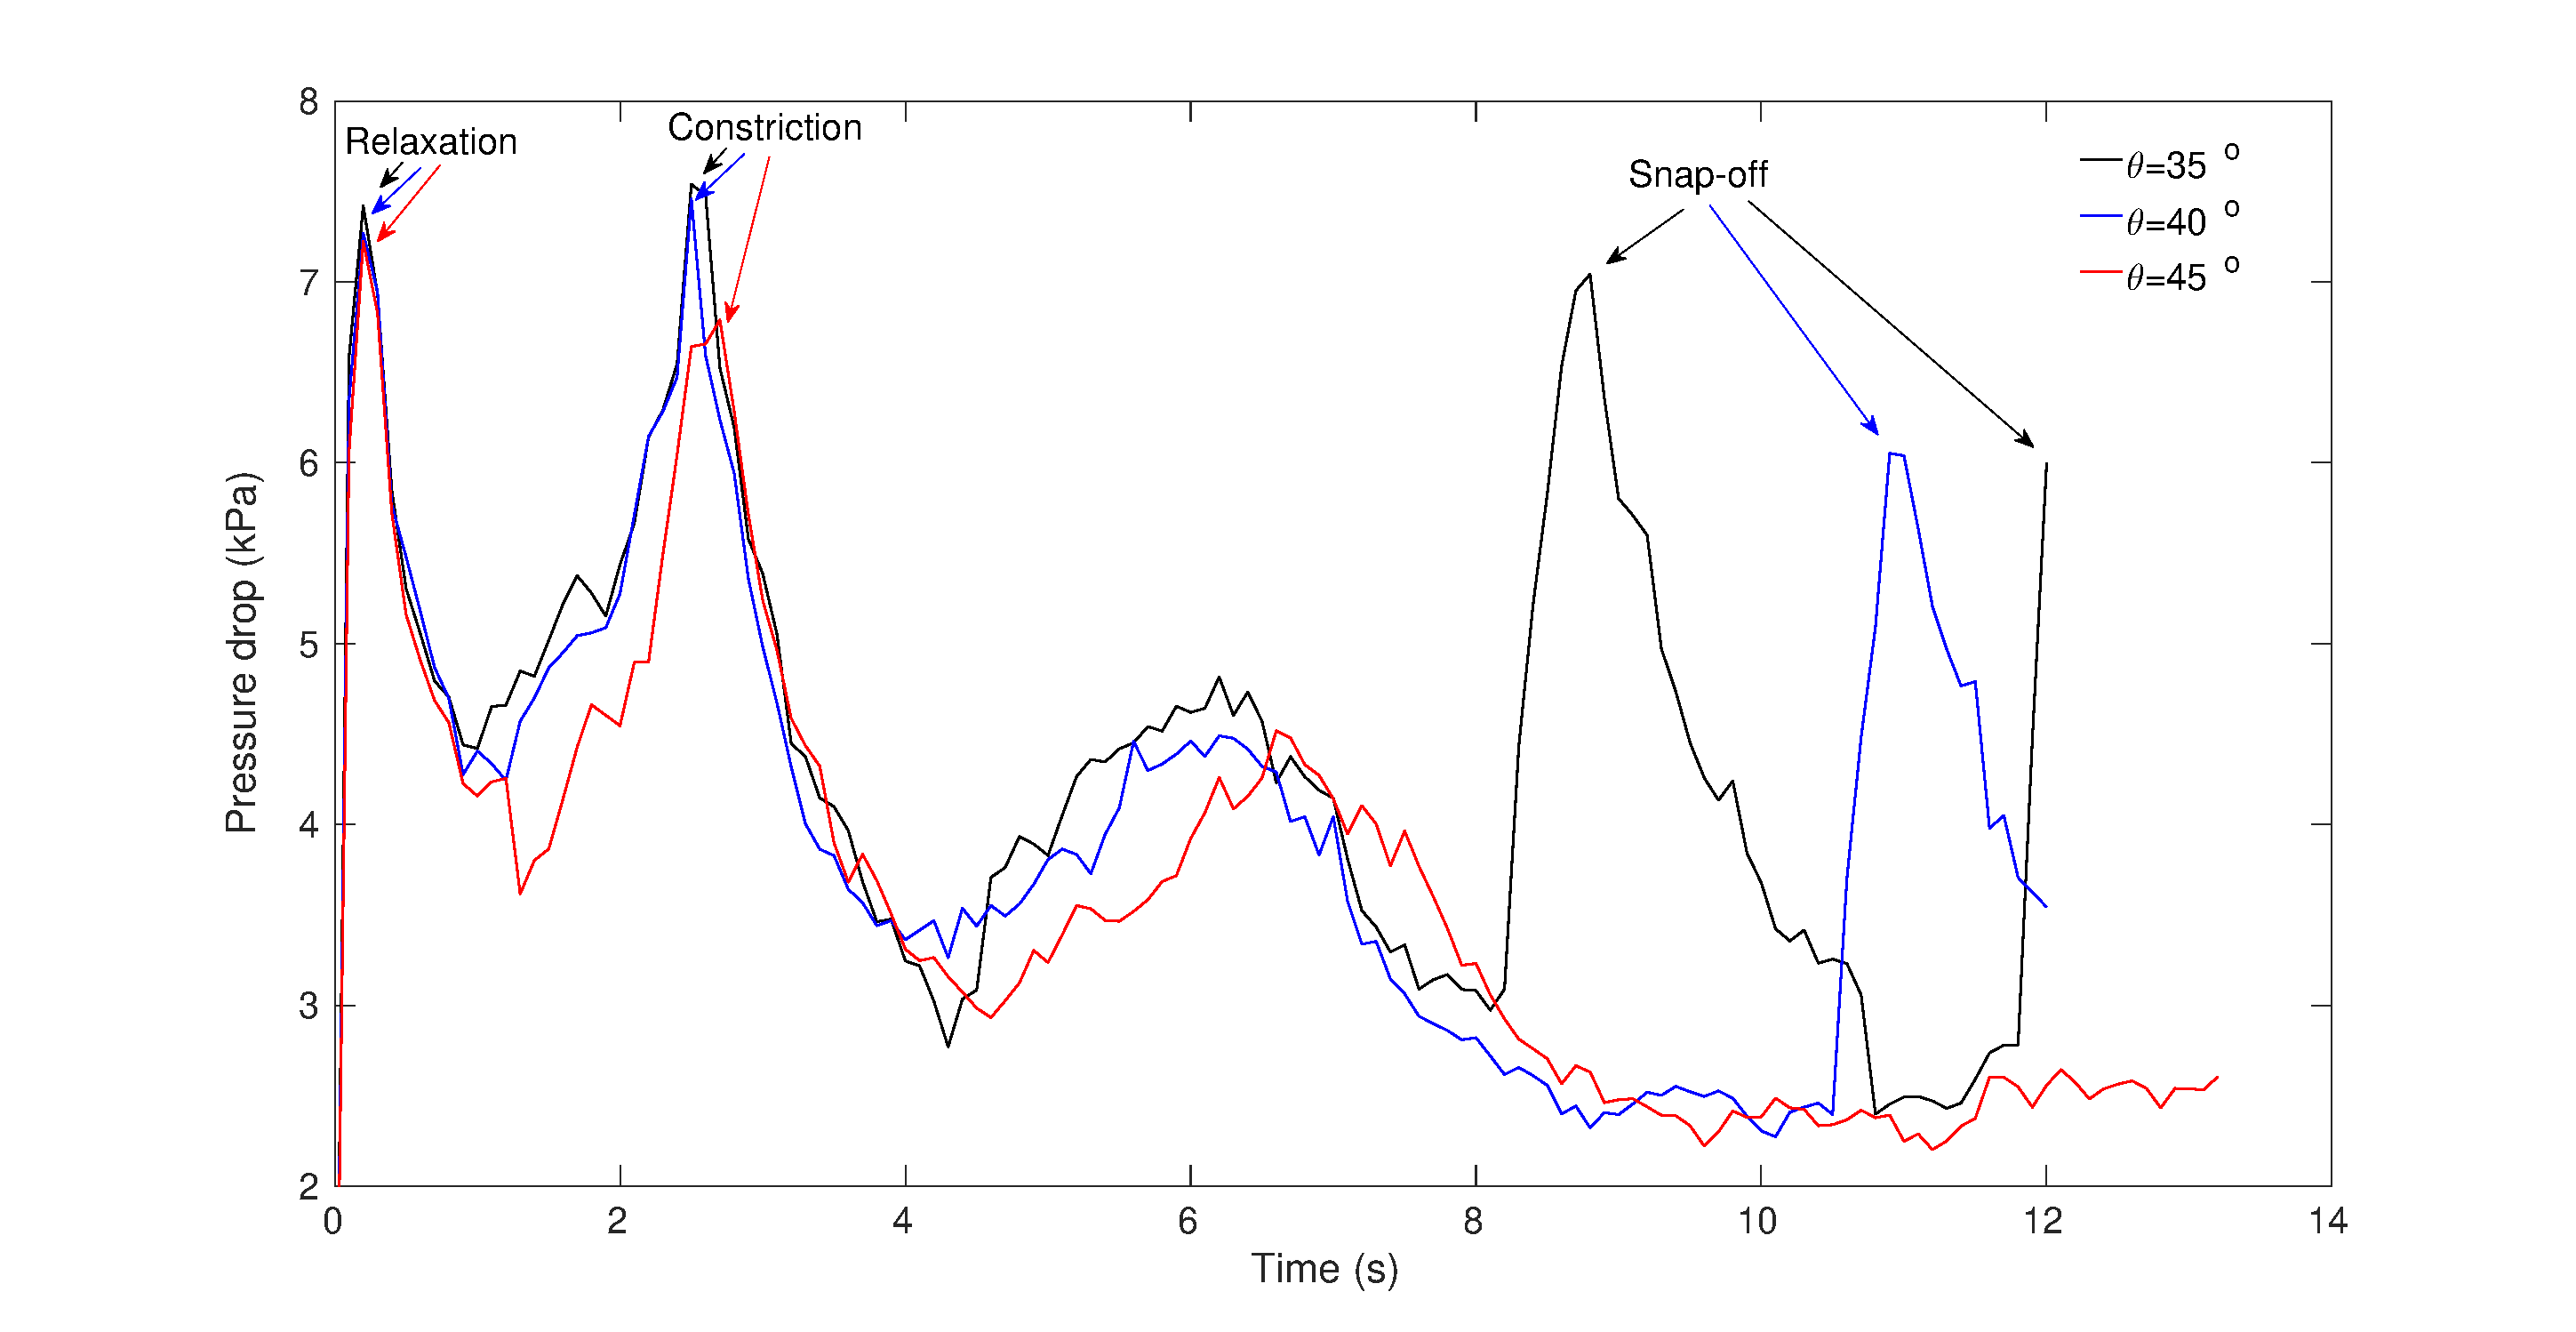
\includegraphics[width=1\textwidth]{\dir/figs/PressureDrop-eps-converted-to.pdf}
    \caption{Caption}   
    \label{pressuredrop}
\end{figure}

The first and second pressure drop peaks are related to stress relaxation (t=0.3s) and throat constriction (t=2.8s) . These two pressure drops can be observed for all three contact angles. Relaxation relates to, when the brine enters the domain, the drop of surface tension due to the capillary equilibrium of interfacial curvature. The second pressure drop peak relates to when the non-wetting fluid invades the throat and lead to the pressure increase. The pressure drop here is the measurement of fluid pressure between inlet and outlet, the outlet fluid pressure is always zero, so when the non-wetting pressure increase so does the pressure drop.

The 35$^\circ$ contact angle curve shows two pressure drop peaks related to snap-off events at t=9s and t=12s. The 40$^\circ$ contact angle curve shows only one pressure drop peak related to snap-off event at t=11s. The 45$^\circ$ curve shows no occurrence of snap-off event. The critical contact angle for the occurrence of snap-off is 43$^\circ$ determined by trail and error step-wisely. 

Fig.\ref{indianasnap} shows the final simulation result of the Roof snap-off event. The total duration of simulation is 12s. The simulation successfully computed the occurrence of the Roof snap-off events, in a similar time scale.

\begin{figure}
    \centering
    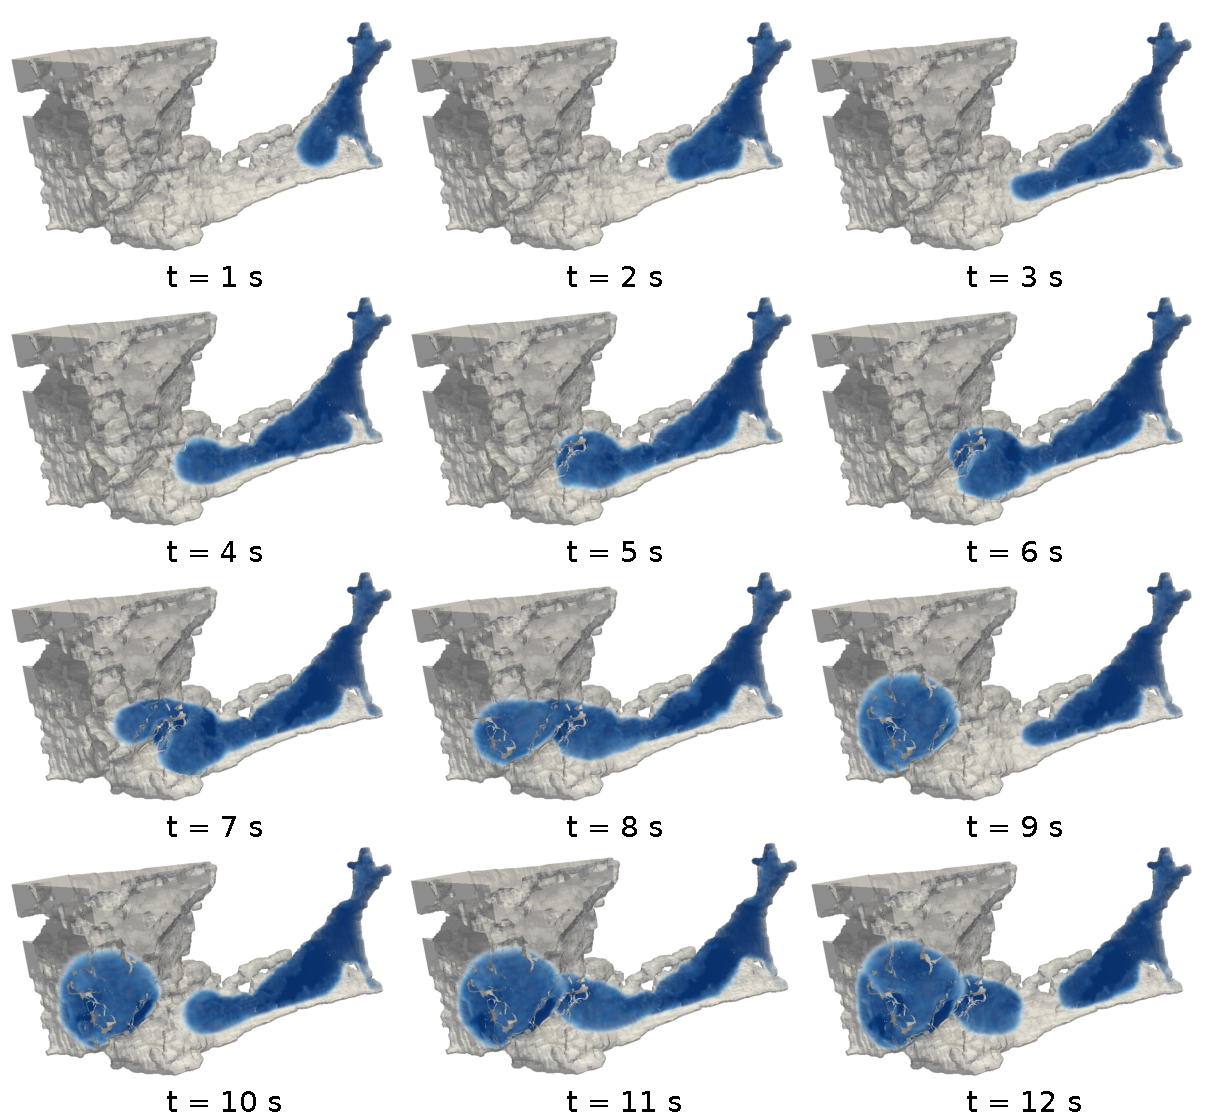
\includegraphics[width=1\textwidth]{\dir/figs/indianasnap-eps-converted-to.pdf}
    \caption{Caption}   
    \label{indianasnap}
\end{figure}


\section{Limitation}
\subsection{Wettability at core perimeter}
In the core-flooding experiments, confining pressure was applied by maintaining constant hydraulic pressure around the core perimeter to approach reservoir pressure conditions. The core was sealed with a heat-shrink sleeve, to separate the core-flooding fluids (brine, oil) and the confining fluid (water). The pores located on the perimeter have one artificial surface that is the heat-shrink sleeve surface. The limitation is caused by different wetting properties of the heat-shrink sleeve with the carbonate core. The heat-shrink sleeves is observed to be non-wetting to the brine, it is yet to be tested on the degree of influence on fluid displacement by the wettability discrepancy. For pore-scale events occurred in these pores, due to this artificial influence of wettability, the displacement events that occurred in these peripheral pores may not be natural. 

Some observations in sub-section \ref{cooperativeporefilling} and \ref{emulsionformationandtrapping} are in these peripheral pores, although the observations of pore-scale displacement mechanisms are true and verified with raw CT images, it remains to be tested if these mechanisms are serendipity due to the artificial surface or they can naturally and commonly occur in the Indiana limestone.

\subsection{Imaging resolution}
The limitations of resolution exist in both spatial and temporal aspect of the X-ray synchrotron micro CT imaging method. For the temporal aspect, the resolution of 20 seconds per scan with 1 second acquisition time is faster than many of the recent related studies using synchrotron CT (e.g. \citet{ramskill2016fast} (16 mins),\citet{menke2016reservoir} (~45s),\cite{menke2017dynamic} (~45s), \cite{khanamiri2018fluid} (2min)). Nonetheless, it is too slow to capture the on-going pore scale events such as snap-off and Haines-jumps, we are only able to see the before-after of such dynamic events. \citet{berg2013real} imaged Haines-jumps with similar temporal resolution (16.8s), and recognised the before-after images of Haines-jumps, but the pressure drop history shows that each Haines-jump event took only 1-2 seconds to happen, which is much faster than the imaging resolution.

In terms of spatial resolution, the resolution of 2.2 micron per pixel is able to define most of the pore surfaces and fluid surfaces. But for wetting films and layer flow in the sub-resolution crevices and rough surfaces, the existence of such configuration can be inferred from fluid flow patterns, but direct imaging is limited by the spatial resolution of the imaging technique.

\section{Future works}
\subsection{Aspect ratio}
The correlation between the aspect ratio distribution and saturation profile will be investigated and discussed in future works.  Fig.\ref{brinesatu,oilsatu} summarised the saturation profile change with injection process. It remains to be investigated how the pore geometry affect the saturation locally and in bulk. This work will enable deeper insights on fluid saturation in heterogeneous pore network.
 
\subsection{Steady-state injection}
The studied steady-state injection experiment had fluid ratio of wetting to non-wetting equals 1. In future steady-state experiments, a range of varied fluid ratio will be experimented to examine the effect of fluid ratio on saturation and displacement pattern etc. This will increase our understanding on simultaneous fluid flow in heterogeneous porous media.
